\cotefile{105}
\scanpage{2}
\unsure{33} -- NODE E33

\margin{\unsure{S E333}\quad $\vert$}

\unsure{$\mathcal Z_a$}

\diagram{\begin{tikzcd}[row sep=small,column sep=large]
\partial \arrow[r,"\unsure{i}"] \arrow[d,phantom,"\big\vert" description] & I \arrow[d,phantom,"\unsure{0\text{-connexe}}" description] \\
\deleted{\unsure{\operatorname{card}}}(\pi_0\partial)\geq 2 & \\
\deleted{\unsure{0\text{-connexe}}} &
\end{tikzcd}}

\[
\left\{\begin{array}{l}
\varnothing\to e\\[2pt]
\partial\times S^{\unsure{n}}(N)\to I\times S^{\unsure{n}}(N)
\end{array}\right.
\]
\inserted{+ Cônes \unsure{gauches} (compl. droits) sur les précédents (donc ici $\{0\}\to\Delta^1$ \unsure{puis} $\{1\}\to\Delta^1$)}

\uline{$\operatorname{Hom}$}$(\unsure{T},X)$

\uline{Lemme} a) Si $X\to e$ a la propriété RLP \unsure{Rel.} pour $\varnothing\to e$ \uline{et} les $\partial S^{\unsure{n}}(N)\to I\times S^{\unsure{n}}(N)$, $N\in\mathcal N$ (partie infinie de $\mathbf N$), alors $X$ est $W_\infty$-asph.

b) Si $X\to Y$ a la RLP p.r. aux cônes gauches (compl. droits) p.r. aux morphismes précédents, alors $X$ est $W_\infty$-propre (resp. $W_\infty$-lisse).

\uline{Cor.} a) Si $X\to Y$ a la propriété RLP p.r. aux \unsure{imm.} de $\unsure{D|\Delta}$ \deleted{\unsure{imm.}\ \illegible{1}} \inserted{entre catégories \unsure{finies}} \inserted{(compl. \unsure{finies})} \deleted{\illegible{3}}, alors c'est une \unsure{fibration} $W_\infty$-propre (compl. lisse) \inserted{$W_\infty$-fibration \unsure{asphérique}}.

b) Si $f\colon X\to Y$ a la propriété RLP p.r. aux \unsure{imm.} \deleted{\unsure{d'ensembles ordonnés finis}\ \unsure{homol.}\ \illegible{1}} \unsure{de catégories} \inserted{(de cat. finies)} qui sont des $W_\infty$, alors $f$ est $W_\infty$-propre (resp. $W_\infty$-lisse).
S'il a la dite propriété pour les $W_\infty$-cofibrations \inserted{entre cat. finies} \unsure{triviales}, alors \unsure{est} $W_\infty$-parfait.

\mspage{1}

\scanpage{3}
\deleted{
Normalement, on voudrait que
\diagram{\begin{tikzcd}
\uline{\unsure{Ch}}(C) \arrow[r,no head,"p"] & C\times C
\end{tikzcd}}
\unsure{ayant|ait} des propriétés de type ``fibration''. Or

1) au sens catégorique, ce n'est ni une fibration, ni une cofibration --- et \unsure{$=$|même} les \deleted{projections} composés
\[
\uline{$s$}\circ p,\ \uline{$\unsure{b}$}\circ p\colon\ \uline{\unsure{Ch}}(C)-C
\]
ne le sont pas.

2) De $\unsure{\simeq}$, \deleted{\unsure{ni}} $p$ \deleted{\illegible{1}} n'est ni coh. propre, ni coh. lisse.
Peut-être au moins \deleted{\unsure{$p$}} $\uline{s}\circ p$ et $\uline{\unsure{b}}\circ p$ le sont-ils \deleted{\illegible{1}} l'un ou l'autre? Mais ce sont plutôt les props de $p$ lui-même qui est important!

3) Il semblerait que $p$ soit une $W_\infty$-fibration.
(``fibration \unsure{cohomologique}'') C'est une chose à vérifier.

\uline{Question} Les $W_\infty$-fibrations, et la notion correspondante de cofibrations \deleted{\unsure{pour}} \inserted{(pour la L.L.P)}, font-ils une \deleted{des} structure de Quillen sur $(\mathrm{Cat})$?
}
\mspage{2}

\scanpage{4}
\margin{\deleted{\unsure{Ahmed}}}
\mspage{3}

\scanpage{5}
\mspage{1}
$\mathcal A$ a topos

$W\subset\mathrm{Fl}(\mathcal A)$ set of arrows, (\inserted{weakly} saturated i.e.
\margin{a) isom. are in $W$

b) if $f=vu$, and two \unsure{among} $u,v,f$ in $W$, so the third.

c) if \diagram{\begin{tikzcd}X \arrow[r,shift left,"f"] & Y \arrow[l,shift left,"g"]\end{tikzcd}} with $gf=\mathrm{id}_X$, $fg\in W$, then $f,g\in W$}
plus other conditions we are going to list, as we need them.

\deleted{\illegible{1}} Let moreover \deleted{$C_0\subset(TC)_0$}
\[
(TC)_0\subset C_0\ (\subset\mathrm{Fl}(\mathcal A))
\]
(with no other assumptions for the time being).

\margin{\uline{NB} $C$ stands for ``cofibrations'', $TC$ for ``trivial cofibrations'', $F$ for ``fibrations'', $TF$ for ``trivial fibrations''.}

We define \deleted{$\unsure{TC}$}
\[
TF\subset F\ (\subset\mathrm{Fl}(\mathcal A))
\]
by the right lifting property (RLP) with respect to \deleted{$(TC)_0$} $C_0$ and $(TC)_0$ respectively, and then
\diagram{\begin{array}{ccc}
TC&\subset&C\ (\subset\mathrm{Fl}(\mathcal A))\\
\cup&&\cup\\
(TC)_0&\subset&C_0
\end{array}}
by the \deleted{right} left lifting property \inserted{(LLP)} with respect to $F$ and $TF$ respectively. We have pairs
\diagram{\begin{array}{cc|cc}
TC&\leftarrow&\rightarrow&F\\
\cap&&&\cup\\
C&\leftarrow&\rightarrow&TF
\end{array}}
in which each \inserted{class} determines the other by RLP \deleted{\unsure{ou}} or LLP. \deleted{Moreover} Moreover

a) $F,TF$ stable by composition, base change, direct factors

b) $C,TC$ stable by composition, \unsure{cobase} change, direct factors
\mspage{4}

\scanpage{6}
\texttt{ACCOUNT NUMBER *********,000000000\quad DATE = 82.160\quad TIME =}

\texttt{JOBNAME= PREDONTA\quad NUMBER=160J0365CNU\quad CPU TOTAL=\quad 15}

\diagram{\begin{array}{@{*}r@{*}l@{*}r@{*}r@{*}r@{*}r@{*}r@{*}r@{*}r@{*}l}
\multicolumn{10}{l}{\texttt{********************************************************************}}\\
\multicolumn{2}{@{*}c@{*}}{}&\multicolumn{2}{c@{*}}{}&\multicolumn{6}{l}{}\\
\multicolumn{2}{@{*}c@{*}}{\mathtt{S\ T\ E\ P}}&\multicolumn{2}{c@{*}}{\mathtt{T\ I\ M\ E}}&\multicolumn{6}{l}{\mathtt{N\ U\ M\ B\ E\ R\quad O\ F}}\\
\multicolumn{2}{@{*}c@{*}}{}&\multicolumn{2}{c@{*}}{}&\multicolumn{6}{l}{}\\
\multicolumn{10}{l}{\texttt{********************************************************************}}\\
&&&&&&&&&\\
\mathtt{NO}&\mathtt{CORE}&\mathtt{TIO}&\mathtt{TCPU}&3330&\mathtt{3330\text{-}1}&3340&3350&2250&\mathtt{T/7TRK}\\
&&&&&&&&&\\
\multicolumn{10}{l}{\texttt{********************************************************************}}\\
&&&&&&&&&\\
1&84&18&14&1&3&0&0&0&0\\
&&&&&&&&&\\
\multicolumn{10}{l}{\texttt{********************************************************************}}\\
\multicolumn{2}{@{*}l@{*}}{}&&&&&&&&\\
\multicolumn{2}{@{*}l@{*}}{\mathtt{TOTALS}}&18&14&1&3&0&0&0&0\\
\multicolumn{2}{@{*}l@{*}}{}&&&&&&&&\\
\multicolumn{10}{l}{\texttt{********************************************************************}}
\end{array}}

\diagram{\begin{array}{@{*}r@{*}l@{*}l@{*}r@{*}r@{*}r@{*}r@{*}r@{*}r@{*}l}
\multicolumn{10}{l}{\texttt{********************************************************************}}\\
\multicolumn{5}{@{*}c@{*}}{}&\multicolumn{2}{c@{*}}{}&\multicolumn{3}{l}{}\\
\multicolumn{5}{@{*}c@{*}}{\mathtt{S\quad T\quad E\quad P}}&\multicolumn{2}{c@{*}}{\mathtt{PAGING}}&\multicolumn{3}{l}{\mathtt{S\ W\ A}}\\
\multicolumn{5}{@{*}c@{*}}{}&\multicolumn{2}{c@{*}}{}&\multicolumn{3}{l}{}\\
\multicolumn{10}{l}{\texttt{********************************************************************}}\\
&&&&&&&&&\\
\mathtt{NO}&\mathtt{NAME}&\mathtt{P\ G\ M}&\mathtt{C.C.U}&\mathtt{SRB}&\mathtt{IN}&\mathtt{OUT}&\mathtt{N}&\mathtt{P.OUT}&\unsure{\mathtt{P}}\\
&&&&&&&&&\\
\multicolumn{10}{l}{\texttt{********************************************************************}}\\
&&&&&&&&&\\
1&\mathtt{CSSBATCH}&\mathtt{CRBATCH}&163&1&0&0&0&0&\\
&&&&&&&&&\\
\multicolumn{10}{l}{\texttt{********************************************************************}}\\
\multicolumn{3}{@{*}c@{*}}{}&&&&&&&\\
\multicolumn{3}{@{*}c@{*}}{\mathtt{T\ O\ T\ A\ L\ S}}&400&1&0&0&0&0&\\
\multicolumn{3}{@{*}c@{*}}{}&&&&&&&\\
\multicolumn{10}{l}{\texttt{********************************************************************}}
\end{array}}

\texttt{RESOURCES ESTIMATED\quad ( SYSOUT = 0120000\quad EXCP =\quad 1000\quad TIME =}

\texttt{RESOURCES USED\quad ( SYSOUT = 0001271\quad EXCP =\quad 4\quad TIME =}

\texttt{\$HASP399 ENDED}
\mspage{5}

\scanpage{7}
\mspage{2}
c) \deleted{$X\to Y$ is $\in W$}
\[
\begin{aligned}
TC&=C\cap\widetilde W\\
TF&=F\cap\widetilde W
\end{aligned}
\]
where
\[
\begin{gathered}
\widetilde W\subset\mathrm{Fl}(\mathcal A)\\
\Vert\\
\{f=pi\mid p\in TF,\ i\in TC\}
\end{gathered}
\]

\uline{NB} These facts do only make use of the existence of finite amalgamated sums and fibred products in $\mathcal A$ (not of the fact that $\mathcal A$ is a topos, --- and for the time being: $W$ has not been used).
We used only the symmetric relationship between \deleted{\unsure{the}} $(TC,F)$ and $(C,TF)$, \deleted{not} plus $TC\subset C$ ($\Leftrightarrow TF\subset F$), not the way they were obtained by some \inserted{pair} $(TC)_0\subset C_0$.

d) \deleted{Assume $TC$, If $i\in C$, $f\in\unsure{F}$} \inserted{consider \deleted{\unsure{let}}, for any}
\[
i\colon A\to B\qquad f\colon X\to Y
\]
\deleted{$i\in C$}\qquad\deleted{$f\in F$}

\deleted{consider}
\diagram{\begin{tikzcd}[column sep=large]
\uline{\mathrm{Hom}}(B,X) \arrow[r,"\uline{\alpha}(i,f)"] & \uline{\mathrm{Hom}}(i,f)\overset{\mathrm{def}}=\uline{\mathrm{Hom}}(B,Y)\mathbin{\times}_{\uline{\mathrm{Hom}}(A,Y)}\uline{\mathrm{Hom}}(A,\unsure{X})
\end{tikzcd}}

\deleted{Then $\alpha(i,f)\in\unsure{F}$}
Then we have the following \deleted{equivalences}
\diagram{\begin{array}{cl}
\left\{\begin{array}{l}\mathrm{(i)}\\[4pt]\mathrm{(ii)}\end{array}\right.
&\begin{array}{l}
C,TC\ \text{stable by cartesian products }?\times\unsure{Z|T}\\[4pt]
TF,\deleted{\unsure{T}}F\ \text{stable by }\uline{\mathrm{Hom}}(\unsure{Z|T},?)
\end{array}\\
\unsure{\Downarrow}&
\end{array}}
\margin{under suitable assumptions}
(iii) If $i\in C$, $f\in F$, then $\alpha(i,f)\in F$, and if moreover $i\in TC$ or $f\in TF$, then $\alpha(i,f)\in TF$.
\mspage{6}

\scanpage{8}
\texttt{9.14.21\quad SYSTEM 370/081 E333\quad VS2 03.8G}

\texttt{RATE = 0, 1}

\diagram{\begin{array}{@{*}r@{*}r@{*}r@{*}r@{*}r@{*}r@{*}r@{*}}
\multicolumn{7}{l}{\texttt{****************************************************}}\\
\multicolumn{4}{l@{*}}{}&\multicolumn{2}{c@{*}}{}&\\
\multicolumn{4}{l@{*}}{\mathtt{E\ X\ C\ P\ S}}&\multicolumn{2}{c@{*}}{\mathtt{BYTES}}&\\
\multicolumn{4}{l@{*}}{}&\multicolumn{2}{c@{*}}{}&\\
\multicolumn{7}{l}{\texttt{****************************************************}}\\
 &  &  &  &  &  & \\
\mathtt{T/8\text{-}16}&\mathtt{T/6250}&\mathtt{SPOOL}&\mathtt{VIO}&\mathtt{SYSIN}&\mathtt{SYSOUT}&\mathtt{C.U}\\
 &  &  &  &  &  & \\
\multicolumn{7}{l}{\texttt{****************************************************}}\\
 &  &  &  &  &  & \\
0&0&1&0&526&\mathtt{0001271}&163\\
 &  &  &  &  &  & \\
\multicolumn{7}{l}{\texttt{****************************************************}}\\
 &  &  &  &  &  & \\
0&0&1&0&526&\mathtt{0001271}&163\\
 &  &  &  &  &  & \\
\multicolumn{7}{l}{\texttt{****************************************************}}
\end{array}}

\diagram{\begin{array}{r@{*}r@{*}r@{*}r@{*}r@{*}r@{*}r@{*}r@{*}r@{*}r@{*}}
\multicolumn{10}{l}{\texttt{****************************************************}}\\
&\multicolumn{2}{c@{*}}{}&\multicolumn{2}{c@{*}}{}&\multicolumn{4}{c@{*}}{}&\\
\mathtt{P}&\multicolumn{2}{c@{*}}{\mathtt{V\ I\ O}}&\multicolumn{2}{c@{*}}{\mathtt{CORE}}&\multicolumn{4}{c@{*}}{\mathtt{S\ E\ T\ U\ P}}&\mathtt{TIME}\\
&\multicolumn{2}{c@{*}}{}&\multicolumn{2}{c@{*}}{}&\multicolumn{4}{c@{*}}{}&\\
\multicolumn{10}{l}{\texttt{****************************************************}}\\
 &  &  &  &  &  &  &  &  & \\
\unsure{\mathtt{P}}\mathtt{.IN}&\mathtt{P.IN}&\mathtt{P.OUT}&\mathtt{TOT}&\mathtt{TOP}&\mathtt{DU}&\mathtt{DM}&\mathtt{TU}&\mathtt{TM}&\mathtt{ELAPS}\\
 &  &  &  &  &  &  &  &  & \\
\multicolumn{10}{l}{\texttt{****************************************************}}\\
 &  &  &  &  &  &  &  &  & \\
0&0&0&5360&244&0&0&0&0&2\\
 &  &  &  &  &  &  &  &  & \\
\multicolumn{10}{l}{\texttt{****************************************************}}\\
 &  &  &  &  &  &  &  &  & \\
0&0&0&&&&0&&0&2\\
 &  &  &  &  &  &  &  &  & \\
\multicolumn{10}{l}{\texttt{****************************************************}}
\end{array}}

\texttt{6 REGION =\quad 150k )\quad GIVING CLASS/PRIO = Q/ 0}

\texttt{1 REGION =\quad 84k )\quad GIVING CLASS/PRIO = A/14}
\mspage{7}

\scanpage{10}
\mspage{3}
\uline{Proof} $(i)\Rightarrow(ii)$ Assume (i), let $f\colon X-Y$, $f\in F$, prove \deleted{$\uline{\mathrm{Hom}}(T,f)$}
\[
(\uline{\mathrm{Hom}}(T,f)\colon\uline{\mathrm{Hom}}(T,X)-\uline{\mathrm{Hom}}(T,Y))\in F
\]
i.e. RLP with respect to any $i\colon A\to B$ \inserted{in $TC$} --- this amounts to RLP of $f$ with respect to $i\times\mathrm{id}_T\colon A\times T\to B\times T$, OK as this is \inserted{still} in $TC$.
Same for $f\in\unsure{TC|TF}$, using stability of $C$ under $\times T$.

$(ii)\Longrightarrow(i)$ Assume (ii), let $i\colon A\to B$, \deleted{prove} \inserted{in $C$}, prove $i\times T\colon A\times T-B\times T$ is still in $C$, i.e. has \deleted{right} LLP with respect to any $f\in TF$, but this amounts to $i$ having the same with respect to $\uline{\mathrm{Hom}}(T,f)$, which is still in $TF$ by assumption OK.

\deleted{$\unsure{(i)\mathbin{\&}(ii)}\Longrightarrow(iii)$}
\uline{NB} The equivalence $(i)\Leftrightarrow(ii)$ can be further generalized, as a relation between $\unsure{\Phi^*},\unsure{\Phi_*}$ associated by LLP and RLP, when we have two functors $\otimes,\uline{\mathrm{Hom}}$ tied by the Cartan relation
\[
\mathrm{Hom}(A\otimes T,X)\simeq\mathrm{Hom}(A,\uline{\mathrm{Hom}}(T,X)).
\]
Moreover, when we have stability of $\unsure{\Phi^*}$ under \deleted{$\unsure{?\otimes?}\ T\otimes?$} \inserted{$?\otimes T$} \inserted{(where \unsure{$\Phi^*$ is} either $C$ or $TC$)}
\deleted{$\unsure{(i)\mathbin{\&}(ii)}\Longrightarrow\unsure{(iii)}$}
or equivalently of $\unsure{\Phi_*}$ under $\uline{\mathrm{Hom}}(T,?)$, then for $i\colon A\to B$ in $\Phi^*$, $f\colon X-Y$ in $\unsure{\Phi_*}$, we'll have that
\[
\inserted{\uline{$\alpha(i,f)$}}\deleted{\uline{$\mathrm{Hom}(i,f)$}}\deleted{\unsure{$\alpha$}}\colon
\uline{\mathrm{Hom}}(B,X)\to\uline{\mathrm{Hom}}(i,f)
\quad\uline{\text{is in }TF}\inserted{(or in $\Phi_*?$)}.
\]
Indeed, this means it has RLP with respect to any $i'\colon A'-B'$ in $C$ \inserted{[$\Phi^*$]}, i.e.
\[
\mathrm{Hom}(B',\uline{\mathrm{Hom}}(B,X))\to
\mathrm{Hom}(\unsure{i''|i'},\deleted{\unsure{\alpha(i,f)}}\inserted{\uline{\mathrm{Hom}}(\deleted{\unsure{\alpha}}\unsure{i},f)})
\]
is surjective. But \deleted{the first \unsure{hand}} \deleted{\unsure{this can}} \inserted{this can be viewed as}
\[
\deleted{\mathrm{Hom}(B'\otimes B,X)}
\]
\[
\mathrm{Hom}(B'\otimes B,X)\longrightarrow\mathrm{Hom}(\deleted{\unsure{\alpha(i',i)}}\deleted{\unsure{i'\otimes i}}\inserted{i'\boxtimes i},f)
\]
where
\[
\deleted{i'\otimes i\colon A'\otimes A\to B'\otimes B}
\]
\[
i'\boxtimes i\quad\deleted{\unsure{\alpha(i,i')}}\deleted{\unsure{i'\boxtimes i}}\colon\quad
A'\otimes B\amalg_{A'\otimes A}B'\otimes A\longrightarrow B'\otimes B.
\]
\margin{\unsure{Much longer}\ \unsure{more carefully}}
\deleted{and} Thus we have to check that if $i,i'\in\Phi^*$, then $i\boxtimes i'$ is in $\Phi^*$.
\margin{\unsure{and conversely}}
[OK if $\Phi^*$ are monomorphisms, say, and $\otimes={}$cartesian product]

Coming back to case of $(C,TF),(TC,F)$, this shows that if $i\in C$, $f\in TF$, then \deleted{$\unsure{\mathrm{Hom}}$} $\alpha(i,f)$ is in $TF$ --- and if $i$ is in $TC$ and $f$ in $F$ then \deleted{$\unsure{\mathrm{Hom}}$} $\alpha(i,f)$ is in $F$,
\mspage{9}

\scanpage{11}

\texttt{STMT NO. MESSAGE}

\texttt{-}

\texttt{4\quad IEF653I SUBSTITUTION JCL - PGM=CRBATCH,REGION=100K,PARM=}

\texttt{\$HASP373 STARTED - INIT 10 - CLASS Q - SYS E333}

\texttt{IEF236I ALLOC. FOR PREDONTA CSSBATCH}

\texttt{IEF237I 581 ALLOCATED TO STEPLIB}

\texttt{IEF237I 2C9 ALLOCATED TO SYS00052}

\texttt{IEF237I VIO ALLOCATED TO SYSUT1}

\texttt{IEF237I JES2 ALLOCATED TO SYSUDUMP}

\texttt{IEF237I 59F ALLOCATED TO CRJIF}

\texttt{IEF237I JES2 ALLOCATED TO SYSIN}

\texttt{IEF237I 59F ALLOCATED TO SYS00002}

\texttt{IEF237I 59F ALLOCATED TO SYS00001}

\texttt{IEF285I\quad CRAY1.PREDONT.CSS.D82160.T091420.R70\quad CATALOGED}

\texttt{IEF285I\quad VOL SER NOS= CRAY11.}

\texttt{CSS2060 - JOB QUEUED FOR TRANSFER}

\texttt{IEF142I PREDONTA CSSBATCH - STEP WAS EXECUTED - COND CODE 0000}

\texttt{IEF285I\quad CISI.PROD.CSSBATCH.V1.YY01\quad KEPT}

\texttt{IEF285I\quad VOL SER NOS= MVS104.}

\texttt{IEF285I\quad SYSCTLG.VSAC015\quad KEPT}

\texttt{IEF285I\quad VOL SER NOS= SAC015.}

\texttt{IEF285I\quad SYS82160.T091418.RA000.PREDONTA.SYSUT1\quad DELETED}

\texttt{IEF285I\quad JES2.JOB00365.S00102\quad SYSOUT}

\texttt{IEF285I\quad SYS1.CR.JIF\quad KEPT}

\texttt{IEF285I\quad VOL SER NOS= CRAY11.}

\texttt{IEF285I\quad JES2.JOB00365.S10101\quad SYSIN}

\texttt{IEF285I\quad SYSCTLG.VCRAY11\quad KEPT}

\texttt{IEF285I\quad VOL SER NOS= CRAY11.}

\texttt{IEF373I STEP /CSSBATCH/ START 82160.0914}

\texttt{IEF374I STEP /CSSBATCH/ STOP 82160.0914 CPU\quad 0MIN 00.14SEC SRB\quad 0MIN 00.01SEC VIRT\quad 84K SYS\quad 244K}

\texttt{IEF375I JOB /PREDONTA/ START 82160.0914}

\texttt{IEF376I JOB /PREDONTA/ STOP 82160.0914 CPU\quad 0MIN 00.14SEC SRB\quad 0MIN 00.01SEC}
\mspage{10}

\scanpage{12}
\mspage{4}
provided we check that if $i,i'\in TC$ \inserted{(resp. in $C$?)}, then $i'\boxtimes i$ is in $TC$! \inserted{(resp. $C$?)}
But \inserted{if} this is so even if we assume only \uline{one} of the two arrows $i,i'$ in $TC$, the other being in $C$, then we get even that
\[
i\in TC,\ f\in F\Longrightarrow\alpha(i,f)\in TF
\]
and $i\in C$, $f\in F\Rightarrow\alpha(i,f)\in F$.
We just used formally
\[
\alpha(i',\uline{\alpha}(i,f))\simeq\alpha(i'\boxtimes i,f)
\]
\uline{To sum up} we get equivalences
\diagram{\begin{array}{rcl}
C\deleted{\unsure{\otimes TC}}\inserted{\otimes T\subset C}\deleted{\unsure{\otimes T}}&\Longleftrightarrow&TF\ \text{stable by }\uline{\mathrm{Hom}}(T,?)\ ;\\
TC\otimes T\subset TC\deleted{\unsure{\otimes T}}&\Longleftrightarrow&F\ \text{stable by }\uline{\mathrm{Hom}}(T,?)\\
\deleted{C\ \text{stable by }i'\boxtimes i^*}\inserted{C\boxtimes C\subset C}&\Longleftrightarrow&(i\in C,f\in TF\Rightarrow\uline{\alpha}(i,f)\in TF)\\
\deleted{\unsure{TC\boxtimes C}\unsure{C\boxtimes TC}}\inserted{TC\boxtimes TC}\subset TC&\Longleftrightarrow&(i\in TC,f\in F\Rightarrow\uline{\alpha}(i,f)\in\deleted{\unsure{F}}F)\\
TC\boxtimes C\subset TC&\Longleftrightarrow&(i\in C,f\in F\Rightarrow\uline{\alpha}(i,f)\in F)
\end{array}}
\margin{\deleted{\unsure{if}\ \unsure{obviously}}}

\uline{Examp.} \inserted{$\mathcal A$ a topos, $\otimes={}$Cartesian product, $\uline{\mathrm{Hom}}$ the usual \unsure{Hom} \inserted{(\unsure{map Section})},}
\deleted{$\mathcal A$ a topos} $C={}$mono, $(TC)_0={}$monomorphisms of the type
\[
\deleted{\unsure{(B_0\times e)}\unsure{(A_0\times B_0)}}\inserted{(B_0\times e)\cup}(A_0\times I)\overset{i}{\subset}\deleted{\unsure{T\times}}B_0\times I,
\]
where
\[
\unsure{A_0|B_0}\overset{i_0}{\longrightarrow}B_0\quad\text{any mono}
\]
$I$ any \uline{$W$-aspheric object} over $e_{\mathcal A}$ endowed with section $e$.
\margin{given kinds of $I$'s with given sections}

$C$ stable by $?\times T$: trivial, hence $\unsure{F|TF}$ stable by $\uline{\mathrm{Hom}}(T,?)$.
$(TC)_0$ stable by $?\times T$ (replace $i_0$ by $i_0\times\mathrm{id}_T$) hence $F$ stable by $\uline{\mathrm{Hom}}(T,?)$, hence $TC$ stable by $?\times T$.

\deleted{$C$ stable by $i'\boxtimes i$: trivial}
$C\boxtimes C\subset C$: trivial

To check $TC\boxtimes C\subset TC$, $C\boxtimes TC\subset TC$. Consider $i$ defined by $i_0\colon A_0-B_0,I,e$ \inserted{(i.e. $i=\unsure{h(i_0,A_0,B_0)|h(i_0,I,e)}$)} and $i'\colon A'\to B'$, consider the diagram
\diagram{\begin{tikzcd}[column sep=large,row sep=large]
\unsure{A'}\times\unsure{A}\arrow[r,hook]\arrow[d,hook,no head]&B'\times\unsure{A}\arrow[d]\\
\unsure{A'}\times\unsure{B}\arrow[r,hook]&B'\times\unsure{B}=B'\times B_0\times I
\end{tikzcd}}
\mspage{11}

\scanpage{13}
\diagram{\begin{array}{rll}
\texttt{1} & \texttt{//PREDONTA JOB '*********,000000000','\hspace{20ex}',} & \texttt{JOB 0365}\\
\texttt{} & \texttt{// MSGLEVEL=(1,1)} & \texttt{}\\
\texttt{2} & \texttt{//\quad EXEC CSSBATCH} & \texttt{00000040}\\
\texttt{3} & \texttt{XXCSSBATCH PROC REG=100K,P=''} & \texttt{00010000}\\
\texttt{4} & \texttt{XXCSSBATCH EXEC PGM=CRBATCH,REGION=\&REG,PARM=\&P} & \texttt{00020000}\\
\texttt{5} & \texttt{XXSTEPLIB DD DSN=CISI.PROD.CSSBATCH.V1.YY01,DISP=SHR} & \texttt{00030003}\\
\texttt{6} & \texttt{XXSYSUT1 DD DSN=\&\&SYSUT1,UNIT=SYSTSO,SPACE=(TRK,30),DISP=(NEW,DELETE)} & \texttt{00031006}\\
\texttt{7} & \texttt{XXSYSUDUMP DD SYSOUT=*} & \texttt{00040000}\\
\texttt{8} & \texttt{XXCRJIF DD DSN=SYS1.CR.JIF,DISP=SHR} & \texttt{00050000}\\
\texttt{9} & \texttt{XXSYSIN DD DDNAME=CRAYIN} & \texttt{00060000}\\
\texttt{10} & \texttt{//CRAYIN DD *} & \texttt{00000050}\\
\texttt{} & \texttt{//} & \texttt{00000160}
\end{array}}
\mspage{12}

\scanpage{14}
\mspage{5}
\diagram{\begin{tikzcd}[column sep=huge,row sep=huge]
\big((A'\times B_0\times e)\cup(A'\times A_0\times I)\arrow[r]\arrow[d,"h(i_0\times\mathrm{id}_{A'},I,e)"] & \big((B'\times B_0\times e)\cup\big((B'\times A_0)\times I\big)\arrow[d,"h(i_0\times\mathrm{id}_{B'},I,e)"']\\
\underbrace{(A'\times B_0)}\times I\arrow[r,hook]&B'\times B_0\times I
\end{tikzcd}}
\deleted{$A'\times B_0\quad\unsure{A'\,h(i_0)}$}

On trouve
\[
i'\boxtimes(i=h(i_0,I,e))=h(i'\boxtimes i_0,I,e)
\]
\margin{\uline{vérifier un}\ \uline{\unsure{jour}}}
et la formule symétrique, donc \unsure{on gagne}.

\uline{We do not know yet} M1 (factorization of any $f$ as $pi$, with either $i\in C,p\in TF$, or $i\in TC,p\in F$), nor M5 (saturation of $\widetilde W$ --- indeed we need only check a), b), to have a closed model category). The factorization $f=pi$ is the usual argument for constructing injectives, using reasonable properties of existence of \inserted{small} generating set of $\mathcal A$, and of filtering direct limits.
The lifting property may again be axiomatized in terms of $\unsure{\Phi^*},\Phi_*$, in a topos or a more general category --- I'll not for the moment work out this general formulation, and \deleted{be content} I'll assume the factorizability \deleted{\unsure{of $f$}} in the two ways.
\margin{\uline{to work}\ \uline{out}}

We now want to identify $\widetilde W$, and check condition b) of saturation. We want even prove $\widetilde W=W$ --- now it becomes essential to \deleted{\unsure{say}} make clear how the definition of $(TC)_0$ \uline{depends} on $W$, taking as ``bunch'' of \deleted{intervals} all intervals $I$ which are $W$-aspheric over $e$. But this may make a difficulty for factorization;
\mspage{13}

\scanpage{15}
\texttt{J E S 2\quad J O B\quad L O G\quad --\quad S Y S T E M\quad E 3 3 3\quad --\quad N O D E\quad E 3 3}

\texttt{09.14.18 J0365CNU\quad \$ J0365*PREDONTA STARTED - INIT 10 - CLASS Q - SYS E333}

\texttt{09.14.19 J0365CNU\quad DSN CISI.PROD.CSSBATCH.V1.YY01}

\texttt{09.14.21 J0365CNU\quad CSS2060 - JOB QUEUED FOR TRANSFER}

\texttt{09.14.21 J0365CNU\quad SMF RECORD 153-1 (CLOSE) WRITTEN}

\texttt{09.14.22 J0365CNU\quad \$ J0365*PREDONTA ENDED}

\texttt{------ JES2 JOB STATISTICS ------}

\texttt{09 JUN 82 JOB EXECUTION DATE}

\texttt{16 CARDS READ}

\texttt{100 SYSOUT PRINT RECORDS}

\texttt{0 SYSOUT PUNCH RECORDS}

\texttt{0.06 MINUTES EXECUTION TIME}

\mspage{14}

\scanpage{16}
\mspage{6}

because this bunch is not ``small'', we'll therefore take \uline{some} such bunch, and see what we need on it to be able to conclude $\widetilde W=W$.

$\widetilde W\overset{?}{\subset}W$. We are reduced to proving $TC\subset W,TF\subset W$. As $TF$ is defined in terms of $C=\text{monomorphisms}$, the inclusion
\[
\boxed{TF\subset W}
\]
is taken as an axiom on $W$. But in case we get an \inserted{separating} interval $I$ which is $TF$ over $e$ i.e. an injective object, \deleted{\unsure{we may etc.}} this inclusion is equivalent with
\[
\boxed{(I\longrightarrow e)\in UW\quad\text{i.e.}\quad(I\times X-X)\in W\quad\text{for any }X}.
\]
\margin{by \deleted{\unsure{the object}} \inserted{\unsure{simply}} \unsure{modifying|adjoining} \unsure{$\{0,1\}$ in $I$}, \unsure{if there is only one point}. \unsure{namely it can be embedded in an injective} --- but this is \unsure{always} true, because the Lawvere object is injective!!!}

Thus, the axiom is really
\[
\text{\textcircled{1}}\qquad\boxed{(L_{\mathcal A}-e)\in UW}.
\]
\margin{\unsure{Lawvere element}}
\margin{or equivalently $\exists$ \uline{separating interval $I$} with $(I\longrightarrow e)\in UW$}

This implies that any $\underline L$-homotopism is in $W$.
But for \uuline{any} separating interval $\underline I$, it is clear that
\[
f\in TF\Longrightarrow f\text{ is a }I\text{-homotopism}.
\]

Next, we got to prove $TC\subset W$. We need first of all
\[
(TC)_0\subset W.
\]
\diagram{\begin{tikzcd}[column sep=large,row sep=large]
\deleted{\unsure{(B_0\times\{e\})}}\ A_0\times\{\unsure{e|I}\}\arrow[r,hook]\arrow[d,hook,"W"'] & B_0\times\{e\}\arrow[d,hook,"W"']\arrow[dr,"W"] & \\
A_0\times I\arrow[r,hook] & A\arrow[r,hook] & B=B_0\times I
\end{tikzcd}}
\margin{\uline{We need for this}
if $S\overset{i}{\lhook\joinrel\longrightarrow}T$ mono, and $S\overset{g}{\lhook\joinrel\longrightarrow}S'$ mono $\in W$ then
\diagram{\begin{tikzcd}
S\arrow[r,hook,"i"]\arrow[d,hook,"g"']&T\arrow[d,hook,"f"]\\
S'\arrow[r,hook,"i'"']&S'\amalg_S T=T'
\end{tikzcd}}
$f\in W$}

and
\mspage{15}

\scanpage{17}

\diagram{\begin{array}{c@{\quad}l@{\quad}c}
\multicolumn{3}{l}{\texttt{********************************************************************************}}\\
\texttt{*}&\texttt{JESNEWS DU 13/05/1982 C68 CADARACHE}&\texttt{*}\\
\multicolumn{3}{l}{\texttt{********************************************************************************}}\\
\texttt{*}&\texttt{2. LA NUMEROTATION DES JOBS SUR C68 SERA DORENAVANT/LEGEREMENT}&\texttt{*}\\
\texttt{*}&\texttt{DIFFERENTE: FORME NOUVELLE ... JXXXXC68}&\texttt{*}\\
\texttt{*}&\texttt{FORME ANCIENNE ... JOBXXXXC}&\texttt{*}\\
\texttt{*}&\texttt{}&\texttt{*}\\
\texttt{*}&\texttt{NOTA BENE : LA FORME ANCIENNE SUBSISTERA SUR LES AUTRES NOEUDS D EXECU}&\texttt{*}\\
\texttt{*}&\texttt{TION DU RESEAU /JUSQU A CE QU ILS PASSENT A CETTE NOUVELLE}&\texttt{*}\\
\texttt{*}&\texttt{VERSION DE JES2}&\texttt{*}\\
\multicolumn{3}{l}{\texttt{********************************************************************************}}\\
\texttt{*}&\texttt{UTILISATEURS C68 CADARACHE}&\texttt{*}\\
\texttt{*}&\texttt{}&\texttt{*}\\
\texttt{*}&\texttt{MISE EN SERVICE D'UN NOUVEAU VOLUME GAF : CAD520 SAUVEGARDE HEBDO}&\texttt{*}\\
\texttt{*}&\texttt{A PARTIR DU MERCREDI 28 AVRIL 1982.}&\texttt{*}\\
\texttt{*}&\texttt{}&\texttt{*}\\
\multicolumn{3}{l}{\texttt{********************************************************************************}}\\
\texttt{*}&\texttt{FORTRAN VS :}&\texttt{*}\\
\texttt{*}&\texttt{-------------}&\texttt{*}\\
\texttt{*}&\texttt{}&\texttt{*}\\
\texttt{*}&\texttt{MISE EN SERVICE A PARTIR DU 13/05/1982 DU F O R T R A N - V S .}&\texttt{*}\\
\texttt{*}&\texttt{}&\texttt{*}\\
\texttt{*}&\texttt{ATTENTION TAILLE MINIMUN POUR LA COMPILATION 920K}&\texttt{*}\\
\texttt{*}&\texttt{}&\texttt{*}\\
\texttt{*}&\texttt{PROCEDURES STANDARD :}&\texttt{*}\\
\texttt{*}&\texttt{}&\texttt{*}\\
\texttt{*}&\texttt{FORTVC CL CLG ........}&\texttt{*}\\
\texttt{*}&\texttt{}&\texttt{*}\\
\texttt{*}&\texttt{}&\texttt{*}\\
\texttt{*}&\texttt{}&\texttt{*}\\
\texttt{*}&\texttt{}&\texttt{*}\\
\end{array}}

\diagram{\begin{array}{c@{\quad}l@{\quad}c}
\multicolumn{3}{l}{\texttt{*******************************************************************}}\\
\texttt{*}&\texttt{}&\texttt{*}\\
\texttt{*}&\texttt{- J E S N E W S F R 1 -     LE 01/06/82}&\texttt{*}\\
\texttt{*}&\texttt{}&\texttt{*}\\
\texttt{*}&\texttt{-----------------------------------------------------------------}&\texttt{*}\\
\texttt{*}&\texttt{-MISE EN SERVICE DE HSM SUR IBM SACLAY}&\texttt{*}\\
\texttt{*}&\unsure{\texttt{--------------------------------------}}&\texttt{*}\\
\texttt{*}&\texttt{-HSM EST EN FONCTION ET GERE LES VOLUMES DITS 'SANS SAUVEGARDE'}&\texttt{*}\\
\texttt{*}&\texttt{}&\texttt{*}\\
\texttt{*}&\texttt{-----------------------------------------------------------------}&\texttt{*}\\
\texttt{*}&\texttt{}&\texttt{*}\\
\texttt{*}&\texttt{NOTE AUX UTILISATEURS NOS :}&\texttt{*}\\
\texttt{*}&\texttt{---------------------------}&\texttt{*}\\
\texttt{*}&\texttt{LES UTILISATEURS QUI SORTENT DES RESULTATS SUR LE}&\texttt{*}\\
\texttt{*}&\texttt{TERMINAL MP1 DOIVENT INDIQUER DESORMAIS :}&\texttt{*}\\
\texttt{*}&\texttt{}&\texttt{*}\\
\texttt{*}&\texttt{P43.MP1 DANS L'INSTRUCTION     /*JOB}&\texttt{*}\\
\texttt{*}&\texttt{P43/MP1 DANS LES INSTRUCTIONS ROUTE}&\texttt{*}\\
\texttt{*}&\texttt{                            OU SUBMIT}&\texttt{*}\\
\texttt{*}&\texttt{( ET NON PLUS FR1.MP1 OU FR1/MP1)}&\texttt{*}\\
\texttt{*}&\texttt{}&\texttt{*}\\
\multicolumn{3}{l}{\texttt{*******************************************************************}}\\
\end{array}}

\mspage{16}

\scanpage{18}
\mspage{7}

\deleted{\unsure{the fact}} that for any \deleted{interval} $I$ \unsure{in} \deleted{\unsure{our}} in our bunch,
$A\times e\longrightarrow A\times I$ is in $W$ for any $A$, \deleted{\unsure{the} $(e\longrightarrow I)$}.
This is \deleted{\unsure{OK for}} \inserted{equivalent to} saying $A\times I-A$ is in $W$ (using saturation) i.e.
\[
\text{\textcircled{2}}\qquad\boxed{(I-e)\in UW.\quad\text{for any }I\text{ in this bunch}}
\]

We have to prove that by saturating $(TC)_0$ into $TC$, we still remain within $W$. But if we use factorization of
\[
f:\ A\overset{TC}{\lhook\joinrel\longrightarrow}B\qquad f\in TC
\]
as
\[
f=pi:\quad A\underset{TC}{\lhook\joinrel\longrightarrow}\unsure{B'|A'}\underset{\deleted{\unsure{T}}F}{\longrightarrow}B,
\]
\deleted{\unsure{in}}
the map $A\overset{i}{\lhook\joinrel\longrightarrow}B'$ is not only in $TC$, but \inserted{also} in $W$
\[
\text{\textcircled{4}}\quad\boxed{\text{if we assume a property of stability of }W\text{ under \inserted{filtering direct} limits}},
\]
and moreover \deleted{under} of \deleted{stability of \unsure{injections}}
\[
\text{\textcircled{3}}\quad\boxed{\text{monomorphisms in }W\text{ by cobase extensions}}
\]
\margin{\uline{\unsure{to write explicit}}}
(which is anyhow necessary for $W=\widetilde W$). \deleted{We get}

Thus \uline{any} map \inserted{$f$} factors into $pi$, with $p\in F$, $i\in TC\cap W$, and in case $f\in TC$, to conclude $f\in W$, we only have to prove $p\in W$. That we get by lifting property for $(f,p)$: a section $s$ of $B'-B$, such that $sf=i$; then $f$ is a retract of (= direct factor) of $i\in W$,
\margin{\diagram{\begin{tikzcd}[column sep=small,row sep=small]
& B'\arrow[d,"p"',"F"]\\
A\arrow[ur,"i","W\ (\text{and }TC)"'] & B\arrow[l,"f","TC"']\arrow[u,bend right=55,"s"']
\end{tikzcd}}}

Thus we need \deleted{\unsure{4}}
\[
\text{\textcircled{5}}\quad W\text{ stable by direct factors}\quad(\text{\uline{not a consequence of saturation?}})
\]
as a necessary condition for $W=\widetilde W$ (because this will imply we have a closed model structure with $\widetilde W$, \deleted{\unsure{by the}} $\widetilde W$ is stable by retractions). Thus \textcircled{1} to \textcircled{5} imply $\widetilde W\subset W$.
\margin{\diagram{\begin{tikzcd}[column sep=small,row sep=small]
A\arrow[r,hook,"W","i"']\arrow[d,"="'] & \unsure{B'|D'}\arrow[d,"p"',"F"]\\
A\arrow[u,bend left=55,"="']\arrow[r,hook,no head,"f"'] & B\arrow[u,bend right=55,"="']
\end{tikzcd}}}
\mspage{17}

\scanpage{19}
\unsure{Now|Note} to

\diagram{\begin{array}{l@{\qquad}l}
\texttt{/*JOB=PREDONTA,ACCT=*********,ALL=M06}&\texttt{J0365CNU}\\
\texttt{//PREDONTA JOB MSGLEVEL=(1,1)}&\\
\texttt{//\qquad EXEC CSSBATCH}&\texttt{00000040}\\
\texttt{//CRAYIN\quad DD *}&\texttt{00000050}\\
\texttt{//}&\texttt{00000160}\\
\texttt{/*}&
\end{array}}
\mspage{18}

\scanpage{20}
\mspage{8}

We still have to see if $W\subset\widetilde W$. For the opposite inclusion we had to make restrictions \inserted{(in terms of $W$)} on the $I$'s (condition 2), now to get $\widetilde W$ large enough, i.e. $TC$ large enough, we must make assumptions which will ensure that this bunch of $I$'s is large enough --- a natural condition would be that it contains a separating interval. We know already there \deleted{are} \inserted{are} ``eligible'' \uline{separating} intervals, namely $W$-aspheric over $e$ and separating --- such as $L$.
\margin{but this cannot possibly be enough, as it would (taking just $L$ by itself) \deleted{\unsure{it}} give just one possibility \deleted{\unsure{of}} of $F$, hence one \unsure{fixed} particular $W$...}

Let $f\in W$, consider factorization
\[
X\overset{\deleted{\unsure{TC_0}}\inserted{i}}{\longrightarrow}X'\overset{p}{\unsure{-|\longrightarrow}}Y\qquad i\in TC,\ p\in F\quad(\text{or }i\in C,\ p\in TF)
\]
we know already that $i\in W$ (resp. $p\in W$) \deleted{Therefore} $p\in W$ (resp. $i\in W$) --- hence we are reduced to \deleted{the case of $i$} proving either one of the two relations
\[
\begin{aligned}
F\cap W&\subset TF&&\text{(necessary for }W\subset\widetilde W,\text{ as }TF=F\cap\widetilde W)\\
C\cap W&\subset TC&&\text{(id)}
\end{aligned}
\]
which are \deleted{\unsure{only}} equivalent \deleted{\unsure{to the}} clearly to the condition $W\subset\widetilde W$ (or equivalently \deleted{\unsure{W}} $\widetilde W=W$). The second \inserted{[first!]} means that if $f:X-Y$ \inserted{[is in $W$ and]} has the \deleted{\unsure{right}} RLP with respect to $(TC)_0$ i.e. all \inserted{to all} $\unsure{h|\alpha}(\deleted{\unsure{f}}i_0,I,e)$, then it has the RLP even with respect to \uline{all} monomorphisms which are in $W$.
\margin{[????]}

We would like this to hold at least in the following two cases:

\margin{In both cases $\mathcal A=\widehat A$}

a) $W=\underline W_A$ ($\underline W$ a basic localizer), $A$ a (local!) $\underline W$-test category

b) $A=A_0\times T$, \inserted{$\widehat A\simeq\underline{\operatorname{Hom}}(A_0^{\mathrm{opp}},\widehat T)\simeq(A_0\deleted{\unsure{\times}}T)^\wedge$} with $T$ a test category, $W=\underline W_{A/A_0}$ ($\underline W$ a basic localizer), $\underline W_{A/A_0}$ is defined componentwise via $\underline W_T$.
\mspage{19}

\scanpage{21}
\texttt{//*\phantom{000}PREDONTA0365\phantom{00000000}I}

\diagram{\begin{array}{l}
\texttt{\phantom{00000000000}00000000\phantom{000000}00000000\phantom{000000}00000000\phantom{000000}00000000}\\
\texttt{\phantom{000000000}0000000000\phantom{0000}0000000000\phantom{0000}0000000000\phantom{0000}0000000000}\\
\texttt{\phantom{0000000}00\phantom{000000}0000\phantom{00}00\phantom{000000}0000\phantom{00}00\phantom{000000}0000\phantom{00}00\phantom{000000}0000}\\
\texttt{\phantom{000000}00\phantom{00000}00\phantom{0}00\phantom{00}00\phantom{00000}00\phantom{0}00\phantom{00}00\phantom{00000}00\phantom{0}00\phantom{00}00\phantom{00000}00\phantom{0}00}\\
\texttt{\phantom{00000}00\phantom{0000}00\phantom{00}00\phantom{00}00\phantom{0000}00\phantom{00}00\phantom{00}00\phantom{0000}00\phantom{00}00\phantom{00}00\phantom{0000}00\phantom{00}00}\\
\texttt{\phantom{0000}00\phantom{000}00\phantom{000}00\phantom{00}00\phantom{000}00\phantom{000}00\phantom{00}00\phantom{000}00\phantom{000}00\phantom{00}00\phantom{000}00\phantom{000}00}\\
\texttt{\phantom{000}00\phantom{00}00\phantom{0000}00\phantom{00}00\phantom{00}00\phantom{0000}00\phantom{00}00\phantom{00}00\phantom{0000}00\phantom{00}00\phantom{00}00\phantom{0000}00}\\
\texttt{\phantom{00}00\phantom{0}00\phantom{00000}00\phantom{00}00\phantom{0}00\phantom{00000}00\phantom{00}00\phantom{0}00\phantom{00000}00\phantom{00}00\phantom{0}00\phantom{00000}00}\\
\texttt{\phantom{0}0000\phantom{000000}00\phantom{00}0000\phantom{000000}00\phantom{00}0000\phantom{000000}00\phantom{00}0000\phantom{000000}00}\\
\texttt{000\phantom{0000000}00\phantom{00}000\phantom{0000000}00\phantom{00}000\phantom{0000000}00\phantom{00}000\phantom{0000000}00}\\
\texttt{0000000000\phantom{0000}0000000000\phantom{0000}0000000000\phantom{0000}0000000000}\\
\texttt{00000000\phantom{000000}00000000\phantom{000000}00000000\phantom{000000}00000000}
\end{array}}

\diagram{\begin{array}{l}
\texttt{PPPPPPPPPPP\phantom{000}RRRRRRRRRRR\phantom{000}EEEEEEEEEEEE\phantom{00}DDDDDDDDD\phantom{00000}000000000000\phantom{00}NN\phantom{00000000}NN\phantom{00}TTTTTTTTTTTT\phantom{000}AAAAAAAAAA}\\
\texttt{PPPPPPPPPPPP\phantom{00}RRRRRRRRRRRR\phantom{00}EEEEEEEEEEEE\phantom{00}DDDDDDDDDD\phantom{0000}000000000000\phantom{00}NNN\phantom{0000000}NN\phantom{00}TTTTTTTTTTTT\phantom{00}AAAAAAAAAAAA}\\
\texttt{PP\phantom{00000000}PP\phantom{00}RR\phantom{00000000}RR\phantom{00}EE\phantom{000000000000}DD\phantom{0000000}DD\phantom{000}00\phantom{00000000}00\phantom{00}NNNN\phantom{000000}NN\phantom{0000000}TT\phantom{0000000}AA\phantom{00000000}AA}\\
\texttt{PP\phantom{00000000}PP\phantom{00}RR\phantom{00000000}RR\phantom{00}EE\phantom{000000000000}DD\phantom{00000000}DD\phantom{00}00\phantom{00000000}00\phantom{00}NN\phantom{0}NN\phantom{00000}NN\phantom{0000000}TT\phantom{0000000}AA\phantom{00000000}AA}\\
\texttt{PP\phantom{00000000}PP\phantom{00}RR\phantom{00000000}RR\phantom{00}EE\phantom{000000000000}DD\phantom{00000000}DD\phantom{00}00\phantom{00000000}00\phantom{00}NN\phantom{00}NN\phantom{0000}NN\phantom{0000000}TT\phantom{0000000}AA\phantom{00000000}AA}\\
\texttt{PPPPPPPPPPPP\phantom{00}RRRRRRRRRRRR\phantom{00}EEEEEEEE\phantom{000000}DD\phantom{00000000}DD\phantom{00}00\phantom{00000000}00\phantom{00}NN\phantom{000}NN\phantom{000}NN\phantom{0000000}TT\phantom{0000000}AAAAAAAAAAAA}\\
\texttt{PPPPPPPPPPP\phantom{000}RRRRRRRRRRR\phantom{000}EEEEEEEE\phantom{000000}DD\phantom{00000000}DD\phantom{00}00\phantom{00000000}00\phantom{00}NN\phantom{0000}NN\phantom{00}NN\phantom{0000000}TT\phantom{0000000}AAAAAAAAAAAA}\\
\texttt{PP\phantom{000000000000}RR\phantom{0000}RR\phantom{000000}EE\phantom{000000000000}DD\phantom{00000000}DD\phantom{00}00\phantom{00000000}00\phantom{00}NN\phantom{00000}NN\phantom{0}NN\phantom{0000000}TT\phantom{0000000}AA\phantom{00000000}AA}\\
\texttt{PP\phantom{000000000000}RR\phantom{00000}RR\phantom{00000}EE\phantom{000000000000}DD\phantom{00000000}DD\phantom{00}00\phantom{00000000}00\phantom{00}NN\phantom{000000}NNNN\phantom{0000000}TT\phantom{0000000}AA\phantom{00000000}AA}\\
\texttt{PP\phantom{000000000000}RR\phantom{000000}RR\phantom{0000}EE\phantom{000000000000}DD\phantom{0000000}DD\phantom{000}00\phantom{00000000}00\phantom{00}NN\phantom{0000000}NNN\phantom{0000000}TT\phantom{0000000}AA\phantom{00000000}AA}\\
\texttt{PP\phantom{000000000000}RR\phantom{0000000}RR\phantom{000}EEEEEEEEEEEE\phantom{00}DDDDDDDDDD\phantom{0000}000000000000\phantom{00}NN\phantom{00000000}NN\phantom{0000000}TT\phantom{0000000}AA\phantom{00000000}AA}\\
\texttt{PP\phantom{000000000000}RR\phantom{00000000}RR\phantom{00}EEEEEEEEEEEE\phantom{00}DDDDDDDDD\phantom{00000}000000000000\phantom{00}NN\phantom{000000000}N\phantom{0000000}TT\phantom{0000000}AA\phantom{00000000}AA}
\end{array}}

\diagram{\begin{array}{l}
\texttt{****A\phantom{00}START\phantom{0}JOB\phantom{0}365\phantom{0}PREDONTA\phantom{000000000000000000}ROOM\phantom{000000}9.20.10\phantom{0}AM\phantom{0}09\phantom{0}JUN\phantom{0}82\phantom{00}R6.PR1\phantom{0000}SYS\phantom{0}JES2\phantom{0}JOB\phantom{0}365\phantom{0}START\phantom{0}A****}\\
\texttt{****A\phantom{00}START\phantom{0}JOB\phantom{0}365\phantom{0}PREDONTA\phantom{000000000000000000}ROOM\phantom{000000}9.20.10\phantom{0}AM\phantom{0}09\phantom{0}JUN\phantom{0}82\phantom{00}R6.PR1\phantom{0000}SYS\phantom{0}JES2\phantom{0}JOB\phantom{0}365\phantom{0}START\phantom{0}A****}\\
\texttt{****A\phantom{00}START\phantom{0}JOB\phantom{0}365\phantom{0}PREDONTA\phantom{000000000000000000}ROOM\phantom{000000}9.20.10\phantom{0}AM\phantom{0}09\phantom{0}JUN\phantom{0}82\phantom{00}R6.PR1\phantom{0000}SYS\phantom{0}JES2\phantom{0}JOB\phantom{0}365\phantom{0}START\phantom{0}A****}\\
\texttt{****A\phantom{00}START\phantom{0}JOB\phantom{0}365\phantom{0}PREDONTA\phantom{000000000000000000}ROOM\phantom{000000}9.20.10\phantom{0}AM\phantom{0}09\phantom{0}JUN\phantom{0}82\phantom{00}R6.PR1\phantom{0000}SYS\phantom{0}JES2\phantom{0}JOB\phantom{0}365\phantom{0}START\phantom{0}A****}\\
\texttt{****A\phantom{00}START\phantom{0}JOB\phantom{0}365\phantom{0}PREDONTA\phantom{000000000000000000}ROOM\phantom{000000}9.20.10\phantom{0}AM\phantom{0}09\phantom{0}JUN\phantom{0}82\phantom{00}R6.PR1\phantom{0000}SYS\phantom{0}JES2\phantom{0}JOB\phantom{0}365\phantom{0}START\phantom{0}A****}\\
\texttt{****A\phantom{00}START\phantom{0}JOB\phantom{0}365\phantom{0}PREDONTA\phantom{000000000000000000}ROOM\phantom{000000}9.20.10\phantom{0}AM\phantom{0}09\phantom{0}JUN\phantom{0}82\phantom{00}R6.PR1\phantom{0000}SYS\phantom{0}JES2\phantom{0}JOB\phantom{0}365\phantom{0}START\phantom{0}A****}
\end{array}}

\texttt{DERNIERE MISE A JOUR DE JOURNAL: 08-06-82}

\texttt{STAGE FORMATION NLT-CLOTILDE LES 22 ET 23 JUIN}
\mspage{20}

\scanpage{22}
\mspage{9}

Alternative presentation of theory, with possibly slightly less strong result --- as presentation of handy \unsure{ns} conditions on a $W$, so that there should exist a closed model structure on $\mathcal A$, s.th. $C=\text{mono}$, $W=$ the given one, hence $TC=C\cap W$, $F$ defined by \deleted{\unsure{lift}} RLP with respect to $TC=C\cap W$, \inserted{(say $(TC)_*$)} $TF$ (``Mono-injective'' maps) defined by RLP with respect to $C$.
\margin{$(TF=C_*)$}

The problems which remain (as we know \inserted{already} $(TF)^*=(C_*)^*=C$)

\textcircled{a}
\[
F^*=\deleted{\unsure{\text{any}}}((TC)_*)^*=TC
\]
--- and as \deleted{$\unsure{((TC)_*}$} $F^*\subset(TF)^*=C$, this amounts to: any monomorphism which has the LLP with respect to $F$ is in $W$. (A saturation type property of $W$ with respect to monomorphisms)

\textcircled{b} $TF=W\cap F$ --- in terms of the assumptions already made previously upon $W$, we know $TF\subset W$ i.e. $TF\subset W\cap F$, thus the problem is $W\cap F\subset TF$, i.e. any $f\in W$ which has the RLP with respect to $W\cap C$ is in $TF$ i.e. is Mono-injective.

c) Factorization $f=pi$ with either $p\in TF$, $i\in C$ (but this is already known and independent of $W$), or $p\in F$, $i\in TC$ \inserted{and even $i\in C\cap W$} --- and this shouldn't be too hard in terms of 3) and 4) by standard arguments. Thus I'll admit c for the time being.

\textcircled{d} Moreover, I'm interested in the following, quite important for me, dual to 3): If $f\in F:X-Y$, and $(Y'-Y)\in W$, then $(X'-X)\in W$.

For handling \textcircled{a} \textcircled{b} \textcircled{d} presumably I'll have to rely strongly upon factorization c). Thus for a), using factorization of $f=pi$, and using $f\in F^*$ we get a section $s$ of $p$ \deleted{\unsure{f}} s.th. $sf=i$, then $f$ is a retract of $i\in W$, and we win if we assume 5).
\margin{\diagram{\begin{tikzcd}[column sep=small,row sep=small]
& X'\arrow[d,"p\in F"]\\
X\arrow[ur,hook,"i\in W\cap C"]\arrow[r,hook,"f"']&Y\arrow[u,bend right=55,"s"']
\end{tikzcd}}}
\mspage{21}

\scanpage{23}
\texttt{//*\quad PREDONT 0002\quad - \unsure{CRAYI|CRAY1}}

\diagram{\begin{array}{l}
\texttt{PPPPPPPPPPP\phantom{000}RRRRRRRRRRR\phantom{000}EEEEEEEEEEEE\phantom{00}DDDDDDDDD\phantom{00000}000000000000\phantom{00}NN\phantom{00000000}NN\phantom{00}TTTTTTTTTTTT}\\
\texttt{PPPPPPPPPPPP\phantom{00}RRRRRRRRRRRR\phantom{00}EEEEEEEEEEEE\phantom{00}DDDDDDDDDD\phantom{0000}000000000000\phantom{00}NNN\phantom{0000000}NN\phantom{00}TTTTTTTTTTTT}\\
\texttt{PP\phantom{00000000}PP\phantom{00}RR\phantom{00000000}RR\phantom{00}EE\phantom{000000000000}DD\phantom{0000000}DD\phantom{000}00\phantom{00000000}00\phantom{00}NNNN\phantom{000000}NN\phantom{0000000}TT}\\
\texttt{PP\phantom{00000000}PP\phantom{00}RR\phantom{00000000}RR\phantom{00}EE\phantom{000000000000}DD\phantom{00000000}DD\phantom{00}00\phantom{00000000}00\phantom{00}NN\phantom{0}NN\phantom{00000}NN\phantom{0000000}TT}\\
\texttt{PP\phantom{00000000}PP\phantom{00}RR\phantom{00000000}RR\phantom{00}EE\phantom{000000000000}DD\phantom{00000000}DD\phantom{00}00\phantom{00000000}00\phantom{00}NN\phantom{00}NN\phantom{0000}NN\phantom{0000000}TT}\\
\texttt{PPPPPPPPPPPP\phantom{00}RRRRRRRRRRRR\phantom{00}EEEEEEEE\phantom{000000}DD\phantom{00000000}DD\phantom{00}00\phantom{00000000}00\phantom{00}NN\phantom{000}NN\phantom{000}NN\phantom{0000000}TT}\\
\texttt{PPPPPPPPPPP\phantom{000}RRRRRRRRRRR\phantom{000}EEEEEEEE\phantom{000000}DD\phantom{00000000}DD\phantom{00}00\phantom{00000000}00\phantom{00}NN\phantom{0000}NN\phantom{00}NN\phantom{0000000}TT}\\
\texttt{PP\phantom{000000000000}RR\phantom{0000}RR\phantom{000000}EE\phantom{000000000000}DD\phantom{00000000}DD\phantom{00}00\phantom{00000000}00\phantom{00}NN\phantom{00000}NN\phantom{0}NN\phantom{0000000}TT}\\
\texttt{PP\phantom{000000000000}RR\phantom{00000}RR\phantom{00000}EE\phantom{000000000000}DD\phantom{00000000}DD\phantom{00}00\phantom{00000000}00\phantom{00}NN\phantom{000000}NNNN\phantom{0000000}TT}\\
\texttt{PP\phantom{000000000000}RR\phantom{000000}RR\phantom{0000}EE\phantom{000000000000}DD\phantom{0000000}DD\phantom{000}00\phantom{00000000}00\phantom{00}NN\phantom{0000000}NNN\phantom{0000000}TT}\\
\texttt{PP\phantom{000000000000}RR\phantom{0000000}RR\phantom{000}EEEEEEEEEEEE\phantom{00}DDDDDDDDDD\phantom{0000}000000000000\phantom{00}NN\phantom{00000000}NN\phantom{0000000}TT}\\
\texttt{PP\phantom{000000000000}RR\phantom{00000000}RR\phantom{00}EEEEEEEEEEEE\phantom{00}DDDDDDDDD\phantom{00000}000000000000\phantom{00}NN\phantom{000000000}N\phantom{0000000}TT}
\end{array}}

\diagram{\begin{array}{l}
\texttt{\unsure{****A}}\texttt{\phantom{000}END\phantom{000}JOB\phantom{0000}2\phantom{00}PREDONT\phantom{00000}-\phantom{0}CRAY\phantom{0}OUTPUT\phantom{0}-\phantom{00000}ROOM\phantom{0000000}9.20.01\phantom{0}AM\phantom{0}09\phantom{0}JUN\phantom{0}82\phantom{00}R6.PR1\phantom{0000}SYS\phantom{0}JES2\phantom{0}JOB\phantom{0000}2\phantom{0}END\phantom{000}A****}\\
\texttt{****A\phantom{000}END\phantom{000}JOB\phantom{0000}2\phantom{00}PREDONT\phantom{00000}-\phantom{0}CRAY\phantom{0}OUTPUT\phantom{0}-\phantom{00000}ROOM\phantom{0000000}9.20.01\phantom{0}AM\phantom{0}09\phantom{0}JUN\phantom{0}82\phantom{00}R6.PR1\phantom{0000}SYS\phantom{0}JES2\phantom{0}JOB\phantom{0000}2\phantom{0}END\phantom{000}A****}\\
\texttt{****A\phantom{000}END\phantom{000}JOB\phantom{0000}2\phantom{00}PREDONT\phantom{00000}-\phantom{0}CRAY\phantom{0}OUTPUT\phantom{0}-\phantom{00000}ROOM\phantom{0000000}9.20.01\phantom{0}AM\phantom{0}09\phantom{0}JUN\phantom{0}82\phantom{00}R6.PR1\phantom{0000}SYS\phantom{0}JES2\phantom{0}JOB\phantom{0000}2\phantom{0}END\phantom{000}A****}\\
\texttt{****A\phantom{000}END\phantom{000}JOB\phantom{0000}2\phantom{00}PREDONT\phantom{00000}-\phantom{0}CRAY\phantom{0}OUTPUT\phantom{0}-\phantom{00000}ROOM\phantom{0000000}9.20.01\phantom{0}AM\phantom{0}09\phantom{0}JUN\phantom{0}82\phantom{00}R6.PR1\phantom{0000}SYS\phantom{0}JES2\phantom{0}JOB\phantom{0000}2\phantom{0}END\phantom{000}A****}\\
\texttt{****A\phantom{000}END\phantom{000}JOB\phantom{0000}2\phantom{00}PREDONT\phantom{00000}-\phantom{0}CRAY\phantom{0}OUTPUT\phantom{0}-\phantom{00000}ROOM\phantom{0000000}9.20.01\phantom{0}AM\phantom{0}09\phantom{0}JUN\phantom{0}82\phantom{00}R6.PR1\phantom{0000}SYS\phantom{0}JES2\phantom{0}JOB\phantom{0000}2\phantom{0}END\phantom{000}A****}\\
\texttt{****A\phantom{000}END\phantom{000}JOB\phantom{0000}2\phantom{00}PREDONT\phantom{00000}-\phantom{0}CRAY\phantom{0}OUTPUT\phantom{0}-\phantom{00000}ROOM\phantom{0000000}9.20.01\phantom{0}AM\phantom{0}09\phantom{0}JUN\phantom{0}82\phantom{00}R6.PR1\phantom{0000}SYS\phantom{0}JES2\phantom{0}JOB\phantom{0000}2\phantom{0}END\phantom{000}A****}
\end{array}}
\mspage{22}

\scanpage{25}
\mspage{10}

$A$ category

if $\Phi\subset\mathrm{Fl}(A)$, let
\[
\begin{aligned}
\Phi^*&=\{u\in\mathrm{Fl}(A)\mid u\text{ has the LLP with respect to }\Phi\}\\
\Phi_*&=\{u\in\mathrm{Fl}(A),\ \text{\rule{5em}{.3pt}}\ \mathrm{RLP}\ \text{\rule{8em}{.3pt}}\}.
\end{aligned}
\]
$\Phi$ is called left saturated if $\Phi=\Psi^*$ for some $\Psi$, i.e. $\Phi=(\Phi_*)^*$,
\inserted{$\Psi$} right saturated if \deleted{it is} $\Psi=\Phi_*$ for some $\Phi$ i.e. $\Psi=(\Psi^*)_*$.

Left saturation, right saturation,
\[
\Phi\subset\deleted{\Phi}(\Phi_*)^*,\quad \Psi\subset(\Psi^*)_*,
\]
Associations $\Phi\mapsto\unsure{\Phi|\Psi}_*^{\deleted{*}}$, $\Psi\mapsto\unsure{\Psi|\Phi}^{*}_{\deleted{*}}$ are \unsure{order} reversing bijections between left saturated and right saturated subsets.

\margin{Right saturation $\Psi$ $\Rightarrow$ stability by composition, base change, \unsure{retracts}. dually for left saturation.}

The \uline{factorization property} for a pair $(\Phi,\Psi)$ of mutually orthogonal subsets of $\mathrm{Fl}(A)$ $(\Phi\subset\Psi^*\text{ i.e. }\Psi\subset\Phi_*)$, is the property \deleted{that}
\[
\forall f\in\mathrm{Fl}(A)\quad\exists\text{ factorization }f=pi,\quad\text{with }i\in\Phi,p\in\Psi.
\]
\deleted{Let $\unsure{\Phi},\unsure{\Psi}$ be the left and right saturations respectively}

\deleted{\unsure{Prop.}} \deleted{Let}
\uline{Proposition} Assume factorization property holds \inserted{(for orthogonal pair $(\Phi,\Psi)$)}.
Then $\Phi=\Psi^*$ iff $\Phi$ stable by direct factors. Dually $\Psi=\Phi_*$ iff $\Psi$ stable by retractions. Hence $(\Phi,\Psi)$ \unsure{are} dual pair of subsets of $\mathrm{Fl}(A)$ (localizers) iff \deleted{and} \deleted{(they are orthogonal} both $\Phi$ and $\Psi$ are stable by direct factors.

\uline{Quillen pair} $(\Phi,\Psi)$:
\diagram{\begin{array}{l}
\text{dual pair}+\text{factorization}\\
\Updownarrow\\
\text{orthogonal pair}+\text{factorization}+\text{stability of }\Phi,\Psi\text{ by direct factors}.
\end{array}}

\uline{Quillen triple} $(C,F,W)$ with

\deleted{Now let}

a) $W$ saturated \inserted{\deleted{\unsure{weakly}} weakly} \textcircled{M5}

\margin{(Iso in $W$, \deleted{and} and \unsure{stb} \unsure{compos.}) \inserted{and \uline{stab. by direct factors}}}

b) $(C,F\cap W\overset{\mathrm{def}}{=}TF)$ and $(TC\overset{\mathrm{def}}{=}C\cap W,F)$ are Quillen pairs i.e. \textcircled{M1} \textcircled{M2} and stability of $C,F,\deleted{\unsure{TC}}$ \deleted{\unsure{and W}} \inserted{$TC,TF$} \deleted{direct factors} under direct factors (it is enough for $C,F$, provided same holds for \textcircled{$W$}).

\margin{it should not be necessary here to impose the direct factor condition on $W$, if one assumes b)}

\diagram{\begin{array}{ccc}
C&TF&\\
\cup&\cap&W\\
TC&F&
\end{array}}

(hence \deleted{\unsure{if}} $f\in W\Longleftrightarrow f=pi$, $i\in TC$, $\unsure{f|p}\in TF$).

! This implies $W$ is strongly saturated i.e. if $\unsure{\gamma|\rho}_W:A\longrightarrow W^{-1}A$,
\[
f\in W\Longleftrightarrow\unsure{\gamma|\rho}_W(f)\text{ iso}.
\]
\margin{true at any rate if in $A$ finite direct and inverse limits exist (M0)}

\mspage{24}

\scanpage{26}
\mspage{25}

\diagram{\begin{array}{llll}
\texttt{09:14:21}&\texttt{0.0000}&\texttt{CSP}&\\
\texttt{09:14:21}&\texttt{0.0000}&\texttt{CSP}&\unsure{\texttt{**********************************************************************}}\\
\texttt{09:14:21}&\texttt{0.0000}&\texttt{CSP}&\texttt{*\phantom{00000000000000000000000000000000000000000000000000000000000000000000}*}\\
\texttt{09:14:21}&\texttt{0.0000}&\texttt{CSP}&\texttt{*\phantom{00000000000000000000000000000000000000000000000000000000000000000000}*}\\
\texttt{09:14:21}&\texttt{0.0000}&\texttt{CSP}&\texttt{*\phantom{00000000000000000000000000000000000000000000000000000000000000000000}*}\\
\texttt{09:14:21}&\texttt{0.0000}&\texttt{CSP}&\texttt{*\phantom{000000000}GETIA\phantom{0}LE\phantom{0}07\phantom{0}JUIN\phantom{0}1982\phantom{00000000000000000000000000000000000000}*}\\
\texttt{09:14:21}&\texttt{0.0000}&\texttt{CSP}&\texttt{*\phantom{000000000}---------------------\phantom{00000000000000000000000000000000000000}*}\\
\texttt{09:14:21}&\texttt{0.0000}&\texttt{CSP}&\texttt{*\phantom{00}ATTENTION\phantom{000000000000000000000000000000000000000000000000000000000}*}\\
\texttt{09:14:21}&\texttt{0.0001}&\texttt{CSP}&\texttt{*\phantom{00}=========\phantom{000000000000000000000000000000000000000000000000000000000}*}\\
\texttt{09:14:21}&\texttt{0.0001}&\texttt{CSP}&\texttt{*\phantom{00}LES\phantom{0}FICHIERS\phantom{0}NON\phantom{0}ACCEDES\phantom{0}DEPUIS\phantom{0}6\phantom{0}MOIS\phantom{0}SERONT\phantom{0}PURGES\phantom{0}LE\phantom{00000000000}*}\\
\texttt{09:14:21}&\texttt{0.0001}&\texttt{CSP}&\texttt{*\phantom{00}VENDREDI\phantom{0}04\phantom{0}JUIN\phantom{0}1982.\phantom{0}CECI\phantom{0}POUR\phantom{0}LA\phantom{0}CISI\phantom{0}UNIQUEMENT.\phantom{00000000000000}*}\\
\texttt{09:14:21}&\texttt{0.0001}&\texttt{CSP}&\texttt{*\phantom{00000000000000000000000000000000000000000000000000000000000000000000}*}\\
\texttt{09:14:21}&\texttt{0.0001}&\texttt{CSP}&\unsure{\texttt{*====================================================================*}}\\
\texttt{09:14:21}&\texttt{0.0001}&\texttt{CSP}&\texttt{*\phantom{00}RAPPEL\phantom{000000000000000000000000000000000000000000000000000000000000}*}\\
\texttt{09:14:21}&\texttt{0.0001}&\texttt{CSP}&\texttt{*\phantom{00}------\phantom{000000000000000000000000000000000000000000000000000000000000}*}\\
\texttt{09:14:21}&\texttt{0.0001}&\texttt{CSP}&\texttt{*\phantom{00}LES\phantom{0}OPTIONS\phantom{0}ON=\unsure{0|O}\phantom{0}ET\phantom{0}ON=F\phantom{0}DU\phantom{0}COMPILATEUR\phantom{0}FORTRAN\phantom{0}CFT\phantom{0}SONT\phantom{0}TRES\phantom{00000}*}\\
\texttt{09:14:21}&\texttt{0.0001}&\texttt{CSP}&\texttt{*\phantom{00}COUTEUSES\phantom{0}EN\phantom{0}TEMPS\phantom{0}CPU,\phantom{0}L'OPTION\phantom{0}ON=\unsure{0|O}\phantom{0}EMPECHE\phantom{0}TOUTE\phantom{0}VECTORISATION-*}\\
\texttt{09:14:21}&\texttt{0.0002}&\texttt{CSP}&\texttt{*\phantom{00}ELLES\phantom{0}NE\phantom{0}DOIVENT\phantom{0}DONC\phantom{0}UTILISEES\phantom{0}QU'A\phantom{0}BON\phantom{0}ESCIENT.\phantom{00000000000000000}*}\\
\texttt{09:14:21}&\texttt{0.0002}&\texttt{CSP}&\texttt{*\phantom{00000000000000000000000000000000000000000000000000000000000000000000}*}\\
\texttt{09:14:21}&\texttt{0.0002}&\texttt{CSP}&\unsure{\texttt{*--------------------------------------------------------------------*}}\\
\texttt{09:14:21}&\texttt{0.0002}&\texttt{CSP}&\texttt{*\phantom{00}RAPPEL\phantom{0000}POUR\phantom{0}LES\phantom{0}UTILISATEURS\phantom{0}EDF\phantom{0}SEULEMENT\phantom{000000000000000000000}*}\\
\texttt{09:14:21}&\texttt{0.0002}&\texttt{CSP}&\texttt{*\phantom{00}------\phantom{000000000000000000000000000000000000000000000000000000000000}*}\\
\texttt{09:14:21}&\texttt{0.0002}&\texttt{CSP}&\texttt{*\phantom{0000}LES\phantom{0}PARAMETRES\phantom{0}DE\phantom{0}LA\phantom{0}CARTE\phantom{0}JOB\phantom{0}DE\phantom{0}L'ENVELOPPE\phantom{0}IBM\phantom{0}CSSBATCH\phantom{0}SONT\phantom{0}*}\\
\texttt{09:14:21}&\texttt{0.0002}&\texttt{CSP}&\texttt{*\phantom{0000}DE\phantom{0}50K\phantom{0}ET\phantom{0}1\phantom{0}SECONDE\phantom{0}(OBLIGATOIRES)\phantom{000000000000000000000000000000}*}\\
\texttt{09:14:21}&\texttt{0.0002}&\texttt{CSP}&\unsure{\texttt{*\phantom{00000000}-----------------------------\phantom{0000000000000000000000000000000}*}}\\
\texttt{09:14:21}&\texttt{0.0002}&\texttt{CSP}&\texttt{*\phantom{00000000000000000000000000000000000000000000000000000000000000000000}*}\\
\texttt{09:14:21}&\texttt{0.0002}&\texttt{CSP}&\texttt{*\phantom{00000}-RAPPEL\phantom{0}DES\phantom{0}NUMEROS\phantom{0}DE\phantom{0}TELEPHONE\phantom{0}DU\phantom{0}SUPPORT\phantom{0}CRAY\phantom{0}:\phantom{0000000000000}*}\\
\texttt{09:14:21}&\texttt{0.0003}&\texttt{CSP}&\texttt{*\phantom{0000000}.\phantom{0}EDF\phantom{0}CLAMART\phantom{0}:\phantom{0}765-37-38\phantom{000000000000000000000000000000000000}*}\\
\texttt{09:14:21}&\texttt{0.0003}&\texttt{CSP}&\texttt{*\phantom{0000000}.\phantom{0}CISI\phantom{0}SACLAY\phantom{0}:\phantom{0}908-64-87\phantom{000000000000000000000000000000000000}*}\\
\texttt{09:14:21}&\texttt{0.0003}&\texttt{CSP}&\texttt{*\phantom{0000000}.\phantom{0}CISI\phantom{0}RUEIL\phantom{00}:\phantom{0}732-02-73\phantom{0}POSTE\phantom{0}552\phantom{00000000000000000000000000}*}\\
\texttt{09:14:21}&\texttt{0.0003}&\texttt{CSP}&\texttt{*\phantom{00000000000000000000000000000000000000000000000000000000000000000000}*}\\
\texttt{09:14:21}&\texttt{0.0003}&\texttt{CSP}&\texttt{*\phantom{00000000000000000000000000000000000000000000000000000000000000000000}*}\\
\texttt{09:14:22}&\texttt{0.0003}&\texttt{CSP}&\unsure{\texttt{**********************************************************************}}\\
\texttt{09:14:22}&\texttt{0.0003}&\texttt{CSP}&\\
\texttt{09:14:22}&\texttt{0.0003}&\texttt{CSP}&\\
\texttt{09:14:22}&\texttt{0.0003}&\texttt{CSP}&\texttt{\phantom{00000000}CRAY-1S/1000\phantom{000}SERIAL-26\phantom{00000}GETIA-CLAMART\phantom{00000000}06/09/82}\\
\texttt{09:14:22}&\texttt{0.0003}&\texttt{CSP}&\\
\texttt{09:14:22}&\texttt{0.0004}&\texttt{CSP}&\texttt{\phantom{00000000}CRAY-1\phantom{0}OPERATING\phantom{0}SYSTEM\phantom{00000}COS\phantom{0}1.10\phantom{00}ASSEMBLY\phantom{0}DATE\phantom{0}05/11/82}\\
\texttt{09:14:22}&\texttt{0.0004}&\texttt{CSP}&\\
\texttt{09:14:22}&\texttt{0.0004}&\texttt{CSP}&\\
\texttt{09:14:22}&\texttt{0.0005}&\texttt{CSP}&\texttt{JOB,JN=PREDONTA,T=9,TIO=9.}\\
\texttt{09:14:22}&\texttt{0.0009}&\texttt{CSP}&\texttt{ACCOUNT,AC=*********.}\\
\texttt{09:14:22}&\texttt{0.0012}&\texttt{CSP}&\texttt{CFT.}\\
\texttt{09:14:22}&\texttt{0.0015}&\texttt{USER}&\texttt{CF000\phantom{0}-\phantom{0}CFT\phantom{0}VERSION\phantom{0}-\phantom{000}05/10/82\phantom{0}1.09}\\
\texttt{09:14:22}&\texttt{0.0035}&\texttt{USER}&\texttt{CF001\phantom{0}-\phantom{0}COMPILE\phantom{0}TIME\phantom{0}=\phantom{0000}0.0020\phantom{0}SECONDS}\\
\texttt{09:14:22}&\texttt{0.0035}&\texttt{USER}&\texttt{CF002\phantom{0}-\phantom{00000}5\phantom{0}LINES,\phantom{0000000000}5\phantom{0}STATEMENTS}\\
\texttt{09:14:22}&\texttt{0.0036}&\texttt{CSP}&\texttt{LDR.}\\
\texttt{09:14:23}&\texttt{0.0235}&\texttt{USER}&\texttt{LD000\phantom{0}-\phantom{0}BEGIN\phantom{0}EXECUTION}\\
\texttt{09:14:23}&\texttt{0.0236}&\texttt{USER}&\texttt{LT063\phantom{0}-\phantom{00000}STOP\phantom{0000000000}IN\phantom{0}GUTS}\\
\texttt{09:14:23}&\texttt{0.0236}&\texttt{CSP}&\texttt{END\phantom{0}OF\phantom{0}JOB}\\
\texttt{09:14:23}&\texttt{0.0236}&\texttt{CSP}&\\
\texttt{09:14:23}&\texttt{0.0236}&\texttt{CSP}&\\
\texttt{09:14:23}&\texttt{0.0236}&\texttt{CSP}&\\
\texttt{09:14:23}&\texttt{0.0236}&\texttt{CSP}&\texttt{\phantom{00000000}JOBNAME\phantom{0}PREDONT\phantom{0}SQ\phantom{0}30624}\\
\texttt{09:14:23}&\texttt{0.0236}&\texttt{CSP}&\texttt{\phantom{00000000}TIME\phantom{0}EXECUTING\phantom{0}IN\phantom{0}CPU\phantom{0}-\phantom{0}00:00:00.0236}\\
\texttt{09:14:23}&\texttt{0.0237}&\texttt{CSP}&\texttt{\phantom{00000000}TIME\phantom{0}WAITING\phantom{0}TO\phantom{0}EXECUTE\phantom{0}00:00:00.7018}\\
\texttt{09:14:23}&\texttt{0.0237}&\texttt{CSP}&\texttt{\phantom{00000000}TIME\phantom{0}WAITING\phantom{0}FOR\phantom{0}I/O\phantom{0}--\phantom{0}00:00:00.7687}\\
\texttt{09:14:23}&\texttt{0.0237}&\texttt{CSP}&\texttt{\phantom{00000000}MEMORY\phantom{0}USAGE\phantom{0}---\phantom{000}0.02974\phantom{0}MWDS-SEC}\\
\texttt{09:14:23}&\texttt{0.0237}&\texttt{CSP}&\texttt{\phantom{00000000}DISK\phantom{0}BLOCKS\phantom{0}MOVED\phantom{0}-----\phantom{000000}259}\\
\texttt{09:14:23}&\texttt{0.0237}&\texttt{CSP}&\texttt{\phantom{00000000}PHYSICAL\phantom{0}I/O\phantom{0}REQUESTS\phantom{0}-\phantom{000000}32}\\
\end{array}}

\scanpage{27}

\deleted{
$Y$ is Kan

\diagram{\begin{tikzcd}X\arrow[r,"\text{fibration}"']&Y\arrow[phantom,d,"\text{Kan}"]\\&\end{tikzcd}}

$\underline{\mathrm{Hom}}(I,Y)\longrightarrow Y\times Y$ is a Kan fibration (if $Y$ is Kan)

is it a Serre fibration

\[
a\longrightarrow Y\times Y\qquad\alpha,\beta\in Y_a\qquad
\underline{\mathrm{Hom}}_{\alpha,\beta}(I_a,Y_a)\qquad
\underline{\mathrm{Hom}}_{\alpha_b,\beta_b}(I,Y_b)
\]
\rule{.85\linewidth}{.3pt}

\[
\left.\begin{array}{ll}
\text{a)}&\mathrm{Iso}_M\subset W\\
\text{b)}&\text{If }f=vu\text{ and two among }u,v,f\text{ are in }W,\text{ so is the third}
\end{array}\right)\Rightarrow\text{mild saturation}
\]
c) $W$ stable by retraction \deleted{(\unsure{strong}\ \unsure{Kan}}

\margin{but does it imply saturation namely $fg\in W,gf\in W\Longrightarrow f,g\in W$??}

\diagram{\begin{tikzcd}A\arrow[r,shift left,"f"]&B\arrow[l,shift left,"g"]\end{tikzcd}}
\[
fg\in W,\ gf\in W\Longrightarrow f,g\in W\ ?
\]
\[
fg\in W,\ gf\unsure{=|\ne}\mathrm{id}_A\Longrightarrow\unsure{fg|f,g}\in W
\]

\diagram{\begin{tikzcd}A\arrow[r,"{\deleted{\unsure{fg}}\,gf}"]&A\end{tikzcd}}
\diagram{\begin{tikzcd}A\arrow[r,"f"]&B\end{tikzcd}}
\diagram{\begin{tikzcd}B\arrow[r,"fg"]&\unsure{B|D}\end{tikzcd}}
\diagram{\begin{tikzcd}A&B\arrow[l,"f"']\arrow[l,bend right=30,"g"]\end{tikzcd}}
\deleted{$\unsure{f}\,fg$}

\diagram{\begin{tikzcd}A\arrow[r,"{=\,\deleted{\unsure{fg}}}"]&A\end{tikzcd}}
\diagram{\begin{tikzcd}
A\arrow[r,"f"]\arrow[d,"f"']&B\arrow[d,shift left,"="]\\
B\arrow[u,bend left=40,"g"]\arrow[r,"fg","\in W"']&B\arrow[u,shift left]
\end{tikzcd}}
\[
\boxed{\begin{array}{ccc}a)&b)&c_1)\ \deleted{\unsure{c}}\\&&c_2)\\&&c_3)\end{array}}
\]

\diagram{\begin{tikzcd}
A\arrow[r,no head,"f"]\arrow[d,shift left,"i"]&B\arrow[d,shift left,"j"]\\
A'\arrow[u,shift left,"p"]\arrow[r,no head,"f'"]&B'\arrow[u,shift left,"q"]
\end{tikzcd}}
\[
\left|\begin{aligned}
f'i&=jf\\
fp&=qf'\\
pi&=\mathrm{id}_A\\
qj&=\mathrm{id}_B\\
f'&\in W
\end{aligned}\right.\quad\overset{?}{\Longrightarrow}f\in W
\]

\diagram{\begin{tikzcd}A\arrow[d,shift left,"f"]\\\unsure{B|D}\arrow[u,shift left,"g"]\end{tikzcd}}
\[
W\qquad h_W
\]
\[
\begin{aligned}
gf&\underset{h}{\sim}\mathrm{id}_A&&\text{donc }gf\in W\\
fg&\underset{h}{\sim}\mathrm{id}_B&&fg\in W
\end{aligned}
\]

\diagram{\begin{tikzcd}[column sep=small]
&&\unsure{L|\Lambda}\\
&\deleted{\unsure{s}}X\arrow[r,"{\unsure{M|W}}","{\unsure{\infty}}"']&X\arrow[u,"d"]\arrow[dll,bend left=35]\arrow[dll,bend left=55]\\
X\times X\arrow[ur,"{s\,\deleted{\unsure{p}}}"]&&
\end{tikzcd}}

c i) $gf=\mathrm{id}_A$, $fg\in W\Longrightarrow\unsure{fg|f,g}\in W$.

c ii) $gf\in W$, $fg\in W\Longrightarrow f,g\in W$

(iii) $W$ stable \deleted{by \unsure{facteurs}} direct factors

\diagram{\begin{tikzcd}[column sep=small]
\text{c ii)}\arrow[dr,Rightarrow]&&\text{(iii)}\arrow[dl,Rightarrow]\\
&\text{c i)}&
\end{tikzcd}}

\diagram{\begin{tikzcd}[column sep=small]
&\unsure{L|\Lambda}\arrow[dl,no head,"d"']\arrow[dr,no head]&\\
X&&I\times X\unsure{:|=}Y\arrow[ll,"{\unsure{p|2g}}"']\arrow[ll,bend right=25]
\end{tikzcd}}
\diagram{\begin{tikzcd}\unsure{L|\Lambda}\arrow[r,bend left=35,"{\unsure{s|7}}"]&X\arrow[l,"d"']\end{tikzcd}}
}

\mspage{26}

\scanpage{28}
\mspage{10 bis}

\diagram{\begin{tikzcd}X\arrow[r,"f"]&Y\end{tikzcd}}
\[
X,Y\in M_{cf}\qquad f\in F
\]
then $f\in TF\Longleftrightarrow\text{retract property}\Longleftrightarrow$

\inserted{i.e.}

\diagram{\begin{array}{cc}
C&F\cap W=TF\\
\cup&\cap\\
TC=C\cap W&F
\end{array}}
\[
\textcircled{a}\left\{\begin{aligned}C&=(TF)^*\\F&=(TC)_*\end{aligned}\right.
\qquad
\inserted{\textcircled{b}}\deleted{\unsure{a}}\quad
W=\{pi\mid\deleted{p\in TF}\ p\in\underset{\substack{\Vert\\\widetilde{TF}}}{C_*},\ i\in\underset{\substack{\Vert\\\widetilde{TC}}}{F^*}\deleted{\unsure{?}}\}
\]
\[
\Downarrow\qquad
\widetilde{TF}\subset F,\quad \unsure{\overline{TC}|\widetilde{TC}}\subset C
\]
(because $F,C$ saturated) \inserted{\unsure{$F$ and $C$}}

\deleted{
$\left.\begin{aligned}TF&=\widetilde{TF}\\TC&=\overline{TC}\end{aligned}\right\}$ because $TF=F\cap W$, $TC=C\cap W$ are stable under direct factors.
[provided we prove $W$ is stable]
}

we only have to \deleted{prove} \inserted{express}, to get b \unsure{in terms} of a), that \deleted{\unsure{$C$}}
\[
\boxed{\widetilde{TF}\subset W,\quad\unsure{\overline{TC}|\widetilde{TC}}\subset W}
\]
and this is equivalent with
\[
\boxed{\widetilde{TF}=TF,\quad\unsure{\overline{TC}|\widetilde{TC}}=TC}
\]
viz $TF,TC$ saturated i.e. $(C,TF)(TC,F)$ Quillen pairs

! \uline{Equivalent conditions in a model category} (in Quillen's sense)

\deleted{(closed model}

(i) satisfies \textcircled{a} and \textcircled{b}, i.e closed model category in Quillen's sense

(ii) $(C,TF=F\cap W)$ and $(TC=C\cap W,F)$ are Quillen pairs

(iii) $C,F,W$ are stable under direct factors.

\diagram{\begin{tikzcd}\text{(i)}\arrow[d,Leftrightarrow]\\\text{(ii)}\\\text{(iii)}\arrow[u,Rightarrow]\end{tikzcd}}

but I'm \unsure{in|to} doubt that (i)(ii) (which are equivalent) does imply that $\underline W$ is stable under direct factors. But Quillen proves it even implies $W$ is strongly saturated (i.e. $f\in W$ iff $\unsure{\gamma|\rho}(f)$ iso) --- at least under the assumption that finite direct and inverse limits exist in $M$.

\rule{.9\linewidth}{.3pt}

\margin{general model category}
\diagram{\begin{tikzcd}[column sep=small,row sep=small]
&&X_2\arrow[r,"{C\text{ or }F}","g"']\arrow[drr,dashed,"F"]&Y_2\arrow[dr,"TF"]&&\\
\varnothing\arrow[r,"C"']&X_1\arrow[ur,"TC"]\arrow[dr,"TF"']\arrow[urr,dashed,"C"']&&&Y_1\arrow[r,no head,"F"']&e\\
&&X\arrow[r,"f"]&Y\arrow[ur,"TC"']&&
\end{tikzcd}}
\[
\begin{aligned}
\unsure{\gamma|\rho}(f)\text{ iso}&\Longleftrightarrow\unsure{\gamma|\rho}(g)\text{ iso}\\
f\in W&\Longleftrightarrow g\in W.
\end{aligned}
\]
\margin{$W$ strongly saturated $\Longleftrightarrow$ for $f:X\to Y$, $X,Y\in M_{cf}$, $f\in C$, $\unsure{\gamma|\rho}(f)$ iso $\Longrightarrow f\in W$. $\Longleftrightarrow$ for $f:X-Y$, $X,Y\in M_{cf}$, $f\in F$, $\unsure{\gamma|\rho}(f)$ iso $\Longrightarrow f\in W$.}

\diagram{\begin{array}{lllll}
\texttt{PAGE 1}&\texttt{ON=\unsure{CELMPQRSTV|CFLMPQRSTV}}&\texttt{06/09/82-09:14:22}&\texttt{CFT 1.09(05/10/82)}&\texttt{PAGE 1}
\end{array}}
\diagram{\begin{array}{rrrl}
1&\texttt{1.}&&\texttt{PROGRAM GUTS}\\
2&\texttt{2.}&&\texttt{WRITE(6,1)}\\
3&\texttt{3.}&1&\unsure{\texttt{FORMAT(' BONJOUR')}|\texttt{FORMAT('BONJOUR')}}\\
4&\texttt{4.}&&\texttt{STOP}\\
5&\texttt{5.}&&\texttt{END}
\end{array}}

\mspage{27}

\scanpage{30}
\mspage{11}

To construct any Quillen triple, we may proceed as follows:

Start with \inserted{a localizer} $C\subset\mathrm{Fl}(A)$, \textcircled{a} \uline{$C$ stable} by direct factors, hence a pair $(C,C_*=TF)$ --- we must check \textcircled{b} \uline{factorization condition for the pair} $(C,C_*)$. \deleted{Now} Then $(C,TF)$ is a Quillen pair.

Let next \textcircled{c} $\boxed{W\supset TF}$ any localizer which is \inserted{\textcircled{d}\ \uline{mildly}} \uline{saturated and stable under direct factors}. We now get $TC=C\cap W$ \inserted{$\subset C$}, which is \deleted{\unsure{again}} stable under direct factors. Take $F=(TC)_*$ \inserted{$(\supset TF=C_*)$}, we must check \textcircled{e} \uline{factorization property for the pair} $(TC,F)$ --- then we get that $(TC,F)$ is a Quillen pair. Lastly, we must still check that $TF=F\cap W$, and by c) we know already $TF\subset F\cap W$, we have to check still that $F\cap W\subset TF$. But using factorization $f=pi$, $p\in TF$, $i\in C$, as $f,p\in W$ we get $i\in W$ hence $i\in W\cap C=TC$, hence there exists $s:X'\to X$ \unsure{s} that $si=\mathrm{id}_X$ (retraction of $X'$ upon $X$) and $fs=p$, hence $f$ a retraction of $p$, hence is in $TF$, OK. Thus

\diagram{\begin{tikzcd}
X\arrow[r,"="]\arrow[d,"i"',"\in TC"]&X\arrow[d,"{f\in F}"]\\
X'\arrow[ur,dashed,"s"]\arrow[r,"p"']&Y
\end{tikzcd}}
\diagram{\begin{tikzcd}
X'\arrow[r,"s"]\arrow[d,"p"']&X\arrow[l,bend left=30,"i"]\arrow[d,"f"]\\
Y\arrow[r,shift left,"="]&Y\arrow[l,shift left]
\end{tikzcd}}

\margin{\uline{\unsure{Relations|fractions}}}

\uline{Proposition} In order for a pair $(C,W)$ to correspond to a Quillen triple $(C,F,W)$, it is ns that the following conditions be satisfied
\[
\left\{\begin{array}{ll}
1)&C,W\text{ \uline{stable by direct factors}, }W\text{ mildly saturated}.\\
2)&\text{Factorization condition for }(C,C_*)\text{ and for }(C\cap W,(C\cap W)_*).\\
3)&W\supset TF\overset{\mathrm{def}}{=}C_*
\end{array}\right.
\]

We have to develop mainly a criterion to get factorization.

[In the case of interest to us, we get 1) fine, 3) almost fine (there comes in the ``test''-assumption though), and 2) causes a little technical problem.] \unsure{am} however, more than in factorization conditions, interested in the

\mspage{29}

\scanpage{31}

\diagram{\begin{array}{lllllll}
\texttt{GUTS}&\texttt{PAGE 2}&\texttt{ON=CELMPQRSTV}&\texttt{06/09/82-09:14:22}&\texttt{CFT 1.09(05/10/82)}&\texttt{PAGE 2}&\texttt{GUTS}
\end{array}}

\texttt{TABLE OF STATEMENT NUMBERS (ALL ADDRESSES IN TABLES ARE IN OCTAL)}

\texttt{--------------------------}

\diagram{\begin{array}{rl}
\texttt{NUMBER}&\texttt{USE}\\
1&\texttt{-FN}
\end{array}}

\texttt{(SN=STATEMENT NUMBER, GSN=GENERATED STATEMENT NUMBER)}

\texttt{(FN=FORMAT NUMBER, UNDEF*=UNDEFINED STATEMENT NUMBER)}

\texttt{TABLE OF NAMES ENCOUNTERED (ADDRESS FOR DUMMY ARGUMENT IS THE ARGUMENT NUMBER)}

\texttt{--------------------------}

\diagram{\begin{array}{rllllrllllrllll}
\texttt{ADDRESS}&\texttt{NAME}&\texttt{TYPE}&\texttt{MAIN USAGE}&\texttt{BLOCK}&\texttt{ADDRESS}&\texttt{NAME}&\texttt{TYPE}&\texttt{MAIN USAGE}&\texttt{BLOCK}&\texttt{ADDRESS}&\texttt{NAME}&\texttt{TYPE}&\texttt{MAIN USAGE}&\texttt{BLOCK}\\
&\texttt{\$MAIN}&&\texttt{ENTRY}&&&\texttt{\$WFF}&&\texttt{EXTERNAL}&&12&\texttt{GUTS}&\texttt{R}&\texttt{ENTRY}&\\
&\texttt{\$STOP}&&\texttt{EXTERNAL}&&&\texttt{\$WFI}&&\texttt{EXTERNAL}&&&&&&
\end{array}}

\texttt{BLOCK NAMES AND LENGTHS IN OCTAL}

\diagram{\begin{array}{ll}\texttt{23-GUTS}&\texttt{4-\#TB}\end{array}}

\texttt{BONJOUR}

\mspage{30}

\scanpage{32}
\mspage{12}

following properties (characterizing a \uline{strict} Quillen triple)

4) \deleted{\unsure{A|At} any base change} \inserted{$W$ stable by base changes} by any $g\in F$, and by cobase changes by any $g\in C$.

\deleted{\unsure{g}}

\uline{NB} From my point of view, $W$ is given beforehand in a rather tangible way, by cohomological criteria, which turn out very handy. In Kan's-Quillen's point of view, $W$ was a little more hidden maybe in terms of (say) its structure, they get to it via \deleted{\unsure{a}} the pair $(C,TF)$ and $F\supset TF$ the Kan fibrations, which is a somewhat ad-hoc construction in terms of a certain \deleted{\unsure{g}} a-priori generating set $(TC)_0$ --- corresponding roughly to expressing the \unsure{horn} lifting property. What remains to be understood, in the context say of general test categories, is the relationship between this and the direct description $TC=C\cap W$, \deleted{\unsure{what}} i.e why this is just the \uline{saturation} of $(TC)_0$. Maybe I should have a look at Gabriel-Zisman and their treatment of ``anodyne extensions''.

\mspage{31}

\scanpage{33}
\texttt{//*\quad PREDONT 0002\quad - \unsure{CRAYI|CRAY1}}

\diagram{\begin{array}{l}
\texttt{PPPPPPPPPPP\phantom{000}RRRRRRRRRRR\phantom{000}EEEEEEEEEEEE\phantom{00}DDDDDDDDD\phantom{00000}000000000000\phantom{00}NN\phantom{00000000}NN\phantom{00}TTTTTTTTTTTT}\\
\texttt{PPPPPPPPPPPP\phantom{00}RRRRRRRRRRRR\phantom{00}EEEEEEEEEEEE\phantom{00}DDDDDDDDDD\phantom{0000}000000000000\phantom{00}NNN\phantom{0000000}NN\phantom{00}TTTTTTTTTTTT}\\
\texttt{PP\phantom{00000000}PP\phantom{00}RR\phantom{00000000}RR\phantom{00}EE\phantom{000000000000}DD\phantom{0000000}DD\phantom{000}00\phantom{00000000}00\phantom{00}NNNN\phantom{000000}NN\phantom{0000000}TT}\\
\texttt{PP\phantom{00000000}PP\phantom{00}RR\phantom{00000000}RR\phantom{00}EE\phantom{000000000000}DD\phantom{00000000}DD\phantom{00}00\phantom{00000000}00\phantom{00}NN\phantom{0}NN\phantom{00000}NN\phantom{0000000}TT}\\
\texttt{PP\phantom{00000000}PP\phantom{00}RR\phantom{00000000}RR\phantom{00}EE\phantom{000000000000}DD\phantom{00000000}DD\phantom{00}00\phantom{00000000}00\phantom{00}NN\phantom{00}NN\phantom{0000}NN\phantom{0000000}TT}\\
\texttt{PPPPPPPPPPPP\phantom{00}RRRRRRRRRRRR\phantom{00}EEEEEEEE\phantom{000000}DD\phantom{00000000}DD\phantom{00}00\phantom{00000000}00\phantom{00}NN\phantom{000}NN\phantom{000}NN\phantom{0000000}TT}\\
\texttt{PPPPPPPPPPP\phantom{000}RRRRRRRRRRR\phantom{000}EEEEEEEE\phantom{000000}DD\phantom{00000000}DD\phantom{00}00\phantom{00000000}00\phantom{00}NN\phantom{0000}NN\phantom{00}NN\phantom{0000000}TT}\\
\texttt{PP\phantom{000000000000}RR\phantom{0000}RR\phantom{000000}EE\phantom{000000000000}DD\phantom{00000000}DD\phantom{00}00\phantom{00000000}00\phantom{00}NN\phantom{00000}NN\phantom{0}NN\phantom{0000000}TT}\\
\texttt{PP\phantom{000000000000}RR\phantom{00000}RR\phantom{00000}EE\phantom{000000000000}DD\phantom{00000000}DD\phantom{00}00\phantom{00000000}00\phantom{00}NN\phantom{000000}NNNN\phantom{0000000}TT}\\
\texttt{PP\phantom{000000000000}RR\phantom{000000}RR\phantom{0000}EE\phantom{000000000000}DD\phantom{0000000}DD\phantom{000}00\phantom{00000000}00\phantom{00}NN\phantom{0000000}NNN\phantom{0000000}TT}\\
\texttt{PP\phantom{000000000000}RR\phantom{0000000}RR\phantom{000}EEEEEEEEEEEE\phantom{00}DDDDDDDDDD\phantom{0000}000000000000\phantom{00}NN\phantom{00000000}NN\phantom{0000000}TT}\\
\texttt{PP\phantom{000000000000}RR\phantom{00000000}RR\phantom{00}EEEEEEEEEEEE\phantom{00}DDDDDDDDD\phantom{00000}000000000000\phantom{00}NN\phantom{000000000}N\phantom{0000000}TT}
\end{array}}

\diagram{\begin{array}{l}
\texttt{****A\phantom{000}START\phantom{000}JOB\phantom{0000}2\phantom{00}PREDONT\phantom{00000}-\phantom{0}CRAY\phantom{0}OUTPUT\phantom{0}-\phantom{00000}ROOM\phantom{0000000}9.19.44\phantom{0}AM\phantom{0}09\phantom{0}JUN\phantom{0}82\phantom{00}R6.PR1\phantom{0000}SYS\phantom{0}JES2\phantom{0}JOB\phantom{0000}2\phantom{0}START\phantom{000}A****}\\
\texttt{****A\phantom{000}START\phantom{000}JOB\phantom{0000}2\phantom{00}PREDONT\phantom{00000}-\phantom{0}CRAY\phantom{0}OUTPUT\phantom{0}-\phantom{00000}ROOM\phantom{0000000}9.19.44\phantom{0}AM\phantom{0}09\phantom{0}JUN\phantom{0}82\phantom{00}R6.PR1\phantom{0000}SYS\phantom{0}JES2\phantom{0}JOB\phantom{0000}2\phantom{0}START\phantom{000}A****}\\
\texttt{****A\phantom{000}START\phantom{000}JOB\phantom{0000}2\phantom{00}PREDONT\phantom{00000}-\phantom{0}CRAY\phantom{0}OUTPUT\phantom{0}-\phantom{00000}ROOM\phantom{0000000}9.19.44\phantom{0}AM\phantom{0}09\phantom{0}JUN\phantom{0}82\phantom{00}R6.PR1\phantom{0000}SYS\phantom{0}JES2\phantom{0}JOB\phantom{0000}2\phantom{0}START\phantom{000}A****}\\
\texttt{****A\phantom{000}START\phantom{000}JOB\phantom{0000}2\phantom{00}PREDONT\phantom{00000}-\phantom{0}CRAY\phantom{0}OUTPUT\phantom{0}-\phantom{00000}ROOM\phantom{0000000}9.19.44\phantom{0}AM\phantom{0}09\phantom{0}JUN\phantom{0}82\phantom{00}R6.PR1\phantom{0000}SYS\phantom{0}JES2\phantom{0}JOB\phantom{0000}2\phantom{0}START\phantom{000}A****}\\
\texttt{****A\phantom{000}START\phantom{000}JOB\phantom{0000}2\phantom{00}PREDONT\phantom{00000}-\phantom{0}CRAY\phantom{0}OUTPUT\phantom{0}-\phantom{00000}ROOM\phantom{0000000}9.19.44\phantom{0}AM\phantom{0}09\phantom{0}JUN\phantom{0}82\phantom{00}R6.PR1\phantom{0000}SYS\phantom{0}JES2\phantom{0}JOB\phantom{0000}2\phantom{0}START\phantom{000}A****}\\
\texttt{****A\phantom{000}START\phantom{000}JOB\phantom{0000}2\phantom{00}PREDONT\phantom{00000}-\phantom{0}CRAY\phantom{0}OUTPUT\phantom{0}-\phantom{00000}ROOM\phantom{0000000}9.19.44\phantom{0}AM\phantom{0}09\phantom{0}JUN\phantom{0}82\phantom{00}R6.PR1\phantom{0000}SYS\phantom{0}JES2\phantom{0}JOB\phantom{0000}2\phantom{0}START\phantom{000}A****}
\end{array}}
\texttt{DERNIERE MISE A JOUR DE JOURNAL: 08-06-82}

\texttt{STAGE FORMATION NLT-CLOTILDE LES 22 ET 23 JUIN}

\mspage{32}

\scanpage{34}
\mspage{13}
\margin{\uline{Factoriza-tion} \uline{Problem}}
\margin{$\unsure{\Phi_0}$ given, $\unsure{\Phi}$ variable. \deleted{NB we need only $\unsure{\Phi}$}}
$M$ a category, $\Phi_0\subset\mathrm{Fl}(M)$, $\Psi=(\Phi_0^{\deleted{*}})_*$, $\Phi_0\subset\Phi\subset\overline\Phi_0=\Psi^*$, we want to deduce conditions on $\Phi_0,\Phi$ insuring that the pair $(\Phi,\Psi)$ satisfies factorization condition, i.e.
\[
\forall f\in\mathrm{Fl}(M),\quad\exists\text{ factorization }f=pi,\quad i\in\Phi,\quad p\in\Psi.
\]
\margin{NB. we do not use $\Phi\subset\unsure{\overline\Phi_0|\Phi_0}$.}
The idea is to take \inserted{(for given $f$)} all diagrams
\diagram{\begin{tikzcd}
A\arrow[r,"v"]\arrow[d,"g"']&X\arrow[d,"f"]\\
B\arrow[r,"u"']&Y
\end{tikzcd}} $(D)$ with $g\in\Phi_0$
giving rise to
\diagram{\begin{tikzcd}
A\arrow[r,"v"]\arrow[d,"\unsure{a|g}"']\arrow[dr,phantom,"\mathrm{coc}"]&X\arrow[d,"\unsure{i_D|g_D}"]\arrow[dd,bend left=55,"f"]\\
B\arrow[r]&X_D=X\amalg_A B\arrow[d,"p_D"]\\
&Y
\end{tikzcd}}
and to define $\deleted{\unsure{\Sigma_1}(f)}\inserted{X_1(f)}=\deleted{\varinjlim}\coprod_{\text{all }D}(X)\,X_D$ (amalgamated sum under $X$)
so that we get factorization
\diagram{\begin{tikzcd}
X\arrow[r,"i_1(f)"]\arrow[d,"f"']&\deleted{\Sigma}X_1(f)\arrow[dl,"\Sigma_1(f)"]\\
Y&
\end{tikzcd}}
\deleted{with} (hopefully) $i_1(f)\in\Phi$.

For this first step, we need

$a)$ $\Phi_0$ is small (we'll see later how to relax this condition)

$b)$ Amalgamated sums indexed by $I$ with $\operatorname{card}I\leq\operatorname{card}\Phi_0$ exist in $M$, \deleted{and}
\inserted{rather, $\overbrace{\operatorname{card}\Phi_0\times c}^{\sigma}$, where $c$ is $\sup(\operatorname{card}\operatorname{Hom}(A,X)\times\operatorname{card}\operatorname{Hom}(B,Y))$ for $\unsure{u|g}:A\to B$ in $\Phi_0$}

$c)$ $\Phi_{\deleted{\unsure{0}}}$ stable by \inserted{\uline{Composition, and by}} cobase extensions, and \inserted{$(d_0)$} by filtering direct limits \inserted{all} indexed by a set $I$ of cardinality $\leq\operatorname{card}\Phi_0$ \inserted{\unsure{v. thus} $\leq\sigma$}.
\margin{do with \unsure{strengthened}}

We then are making a transfinite induction to define $X_\alpha(f)$ and
\diagram{\begin{tikzcd}
X\arrow[r,"i_\alpha(f)"]\arrow[d,"f"']&X_\alpha(f)\arrow[dl,"\Sigma_\alpha(f)"]\\
Y&
\end{tikzcd}}
$i_\alpha(f)\in\Phi$
with $\alpha$ any ordinal \deleted{$\unsure{\Phi}$} $<\alpha_0$ ($\alpha_0$ \deleted{first} ordinal \deleted{\unsure{of the cardinal}\illegible{2}} \inserted{number to be fixed} \deleted{\unsure{define later in terms of $\pi$}} \inserted{later}).
\[
\left\{\begin{aligned}
\Sigma_{\alpha+1}(f)&=\Sigma_1(\Sigma_\alpha(f)),\quad X_{\alpha+1}(f)=\text{source}\,\Sigma_{\alpha+1}(f),\quad i_{\alpha+1}(f)=\text{composition}\\[4em]
\Sigma_\alpha(f)&=\varinjlim_{\alpha'<\alpha}\Sigma_{\alpha'}(f)\quad\text{if $\alpha$ is a limiting ordinal.}
\end{aligned}\right.
\]
\diagram{\begin{tikzcd}
X\arrow[r,"i_\alpha(f)"]\arrow[d,"f"']&X_\alpha(f)\arrow[r,"i_1(\Sigma_\alpha(f))"]\arrow[dl,"\Sigma_\alpha(f)"]&X_{\alpha+1}(f)\arrow[dll,"\Sigma_{\alpha+1}(f)=\Sigma_1(\Sigma_\alpha(f))"]\\
Y&&
\end{tikzcd}}
\deleted{We} We assume that $\Phi$ is stable too by \inserted{the} filtering direct limits \deleted{of cardinality $\leq c$} which occur in the several transfinite induction steps.
Let $\pi$ be a cardinal such that \deleted{all objects of $\Phi_0$} \inserted{for any $g\in\Phi_0$, source and target of $g$} are $\pi$-\unsure{access. ob.}
--- i.e. $\operatorname{Hom}(A,-):M-\mathrm{Sets}$ commutes to filtering direct limits which are \deleted{\unsure{great wr}} ``large with resp. to $\pi$''. We may take $\pi=\sup_{g\in\Phi_0}\pi_g$, where
\mspage{33}

\scanpage{35}
\diagram{\begin{array}{llllllll}
\mathtt{IMTADE}&\mathtt{IMTAE}&\mathtt{IMTASD}&\mathtt{\unsure{IMTA01|IMTAO1}}&\mathtt{IMTYNO}&\mathtt{IMVISU}&\mathtt{IMVVFR}&\mathtt{IM1BDC}\\
\mathtt{INICSD}&\mathtt{INITMP}&\mathtt{\unsure{INTAR0|INTARO}}&\mathtt{ISNOF5}&\mathtt{LEAMAT}&\mathtt{LEAMMS}&\mathtt{LEATRI}&\mathtt{LEB}\\
\mathtt{LEBDCL}&\mathtt{LECOOR}&\mathtt{LEFORC}&\mathtt{LEHYMA}&\mathtt{LEMAIL}&\mathtt{LEMEFI}&\mathtt{LEMILI}&\mathtt{LEMPLR}\\
\mathtt{LEMUA}&\mathtt{\unsure{LENOPO|LENOP0}}&\mathtt{LETAE}&\mathtt{LETASD}&\mathtt{LETYNO}&\mathtt{LEVISU}&\mathtt{LEVVFR}&\mathtt{LRNDL1}\\
\mathtt{LSVVFR}&\mathtt{\unsure{MONOFO|MONOF0}}&\mathtt{MONOF5}&\mathtt{MONOF6}&\mathtt{NCMUNS}&\mathtt{NDL}&\mathtt{NIVLIB}&\mathtt{NUPAG}\\
\mathtt{NUPAGE}&\mathtt{\unsure{PRINTB|PRINTR}}&\mathtt{\unsure{PRIN1B|PRIN1R}}&\mathtt{\unsure{RACRNO|RACRN0}}&\mathtt{REAMAT}&\mathtt{REATRI}&\mathtt{REB}&\mathtt{REBDCL}\\
\mathtt{RECOOR}&\mathtt{REFORC}&\mathtt{REHYMA}&\mathtt{REMAIL}&\mathtt{REMEFI}&\mathtt{REMILI}&\mathtt{REMPLR}&\mathtt{REMUA}\\
\mathtt{\unsure{RENOPO|RENOP0}}&\mathtt{RESOUR}&\mathtt{RETAE}&\mathtt{RETASD}&\mathtt{RETYNO}&\mathtt{REVISU}&\mathtt{REVVFR}&\mathtt{RSTSDE}\\
\mathtt{SAUCSD}&\mathtt{SAUSDS}&\mathtt{SAUTP}&\mathtt{SDBMSC}&\mathtt{STAMD}&\mathtt{STAMR}&\mathtt{TRAMAD}&\mathtt{TRAMAR}\\
\mathtt{TUERSD}&\mathtt{TUTASD}&\mathtt{VERNN}&\mathtt{VERTNN}&&&&\\\hline
\end{array}}
\deleted{\diagram{\begin{array}{llllllll}
\mathtt{IMAMA1}&\mathtt{IMAMA2}&\mathtt{IMATRI}&\mathtt{IMB}&\mathtt{IMBDCL}&\mathtt{IMB1}&\mathtt{IMCOOR}&\mathtt{\unsure{IMC001|IMCOO1}}\\
\mathtt{IMFORC}&\mathtt{IMHYMA}&\mathtt{IMMAIL}&\mathtt{IMMAI1}&\mathtt{IMMILI}&\mathtt{IMMPLR}&\mathtt{IMMUA}&\mathtt{\unsure{IMNOP0|IMNOPO}}\\
\mathtt{IMTADE}&\mathtt{IMTAE}&\mathtt{IMTASD}&\mathtt{\unsure{IMTA01|IMTAO1}}&\mathtt{IMTYNO}&\mathtt{IMVISU}&\mathtt{IMVVFR}&\mathtt{IM1BDC}\\
\mathtt{INICSD}&\mathtt{INITMP}&\mathtt{\unsure{INTAR0|INTARO}}&\mathtt{ISNOF5}&\mathtt{LEAMAT}&\mathtt{LEAMMS}&\mathtt{LEATRI}&\mathtt{LEB}\\
\mathtt{LEBDCL}&\mathtt{LECOOR}&\mathtt{LEFORC}&\mathtt{LEHYMA}&\mathtt{LEMAIL}&\mathtt{LEMEFI}&\mathtt{LEMILI}&\mathtt{LEMPLR}\\
\mathtt{LEMUA}&\mathtt{\unsure{LENOPO|LENOP0}}&\mathtt{LETAE}&\mathtt{LETASD}&\mathtt{LETYNO}&\mathtt{LEVISU}&\mathtt{LEVVFR}&\mathtt{LRNDL1}\\
\mathtt{LSVVFR}&\mathtt{\unsure{MONOFO|MONOF0}}&\mathtt{MONOF5}&\mathtt{MONOF6}&\mathtt{NCMUNS}&\mathtt{NDL}&\mathtt{NIVLIB}&\mathtt{NUPAG}\\
\mathtt{NUPAGE}&\mathtt{\unsure{PRINTB|PRINTR}}&\mathtt{\unsure{PRIN1B|PRIN1R}}&\mathtt{\unsure{RACRNO|RACRN0}}&\mathtt{REAMAT}&\mathtt{REATRI}&\mathtt{REB}&\mathtt{REBDCL}\\
\mathtt{RECOOR}&\mathtt{REFORC}&\mathtt{REHYMA}&\mathtt{REMAIL}&\mathtt{REMEFI}&\mathtt{REMILI}&\mathtt{REMPLR}&\mathtt{REMUA}\\
\mathtt{\unsure{RENOPO|RENOP0}}&\mathtt{RESOUR}&\mathtt{RETAE}&\mathtt{RETASD}&\mathtt{RETYNO}&\mathtt{REVISU}&\mathtt{REVVFR}&\mathtt{RSTSDE}\\
\mathtt{SAUCSD}&\mathtt{SAUSDS}&\mathtt{SAUTP}&\mathtt{SDBMSC}&\mathtt{STAMD}&\mathtt{STAMR}&\mathtt{TRAMAD}&\mathtt{TRAMAR}\\
\mathtt{TUERSD}&\mathtt{TUTASD}&\mathtt{VERNN}&\mathtt{VERTNN}&&&&
\end{array}}}
\mspage{34}

\scanpage{36}
\mspage{14}
$\pi_g$ is the smallest cardinal s.th. source and target of $g$ are $\pi$-accessible.

\uline{Example} If the objects occurring as sources and targets of $g$'s in $\Phi_0$ are ``of finite presentation'', i.e. $\operatorname{Hom}(A,-)$ commutes with any filtering direct limits, we get $\pi=0$. In this case we stop the induction with $\alpha_0=$ first infinite ordinal \deleted{the first \unsure{one}}. In case the objects $A,B$ are not of finite presentation, (\unsure{still|but} they are accessible
--- we take the smallest cardinal such that $\operatorname{Hom}(A,?)$ commutes with direct limits indexed by \deleted{\unsure{ordi}} directed sets \deleted{great} \inserted{large} w.r. $\pi$.
Let \inserted{then} $\alpha_0$ be the first ordinal s.th. the set
\[
I_{\alpha_0}=\{\text{all ordinals }\alpha\text{ with }\alpha<\alpha_0\}
\]
be \deleted{great} large wrt $\pi$. We take the factorization
\diagram{\begin{tikzcd}
X\arrow[r,"i_{\alpha_0}(f)=i(f)"]\arrow[d]&X_{\alpha_0}(f)=\deleted{\Sigma}\unsure{\overline X}(f)\arrow[dl,"\Sigma_{\alpha_0}(f)=p(f)"]\\
Y&
\end{tikzcd}}
and we get $i(f)\in\Phi$, $p(f)\in\Psi$, provided we make the following assumptions;

$d)$ The \deleted{\unsure{elem}} source and target objects of the arrows of $\Phi_0$ are \uline{accessible}
(ok if $M$ a topos etc ---) and, if $\pi_0$ is the cardinality of the smallest ordinal number \inserted{$\alpha_0$} s.th. for any such $A$, $\operatorname{Hom}(A,-)$ commutes to the direct limits of type $I_{\alpha_0}$, \deleted{\unsure{we}} and \deleted{$\pi=\sup(\unsure{\pi}$}
$\pi=\sup(\pi_0,\operatorname{card}\Phi_0)$ \inserted{rather, $\sigma$}, we assume that for any filtering direct system with an indexing set $I$ of cardinality $\leq\pi$, and transition maps in $\Phi$, the direct limit exists and \deleted{$\unsure{X_n}$} $Z_i\to Z$ are equally in $\Phi$.

Then we get, not only factorization $f=pi$, with $i\in\Phi$, $p\in\Psi$, but even factorization $\uline{\overline X}(f)$ \uline{functorial} with respect to variable $f$.
\mspage{35}

\scanpage{37}
\margin{UTDE\\UTIL\\UTSD}
\texttt{llpd 'cnu1.modulef.utda'}
\diagram{\begin{array}{llllllll}
\mathtt{AFMDES}&\mathtt{CLOSE}&\mathtt{CUTTER}&\mathtt{DYNAM}&\mathtt{ECRDIR}&\mathtt{ECR1}&\mathtt{FLIPFLOP}&\mathtt{INCANO}\\
\mathtt{INCAPA}&\mathtt{INDUNI}&\mathtt{IVIRT}&\mathtt{LAYOUT}&\mathtt{LECDIR}&\mathtt{LEC1}&\mathtt{LISTPDS}&\mathtt{MDES}\\
\mathtt{MESSAGE}&\mathtt{NUMALP}&\mathtt{OPEN}&\mathtt{TRANSLAT}&\mathtt{UPDATE}&&&
\end{array}}
\margin{$\unsure{1|I}$\\$\unsure{B|\beta}$}
\margin{21}
\texttt{llpd 'cnu1.modulef.utdas'}
\diagram{\begin{array}{llllllll}
\mathtt{AFMDES}&\mathtt{CLOSE}&\mathtt{CUTTER}&\mathtt{DYNAM}&\mathtt{ECRDIR}&\mathtt{FLIPFLOP}&\mathtt{INCANO}&\mathtt{INDUNI}\\
\mathtt{IVIRT}&\mathtt{LAYOUT}&\mathtt{LECDIR}&\mathtt{LISTPDS}&\mathtt{MDES}&\mathtt{MESSAGE}&\mathtt{NUMALP}&\mathtt{OPEN}\\
\mathtt{TRANSLAT}&\mathtt{UPDATE}&&&&&&\\\hline
\end{array}}
\margin{$\unsure{\Pi|\Omega}$}
\texttt{llpd 'cnu1.modulef.utde'}
\diagram{\begin{array}{llllllll}
\mathtt{AFMDES}&\mathtt{CLOSE}&\mathtt{CUTTER}&\mathtt{DEFDIR}&\mathtt{DYNAM}&\mathtt{ECPDIR}&\mathtt{ECP1}&\mathtt{ECRDIR}\\
\mathtt{ECRF0}&\mathtt{ECR1}&\mathtt{ECTDIR}&\mathtt{ERLIBR}&\mathtt{FERDIR}&\mathtt{FLIPFLOP}&\mathtt{INCANO}&\mathtt{INCAPA}\\
\mathtt{INDUNI}&\mathtt{INIDIR}&\mathtt{INITI}&\mathtt{IVIRT}&\mathtt{LAYOUT}&\mathtt{LECDIR}&\mathtt{LECTAB}&\mathtt{LECTUD}\\
\mathtt{LECTUI}&\mathtt{LECTUK}&\mathtt{LECTUT}&\mathtt{LECTU1}&\mathtt{LECTU2}&\mathtt{LECTU3}&\mathtt{LECTU4}&\mathtt{LECTU5}\\
\mathtt{LECT10}&\mathtt{LECVAL}&\mathtt{LEC1}&\mathtt{LEPDIR}&\mathtt{LEP1}&\mathtt{LETDIR}&\mathtt{LISTPDS}&\mathtt{MDES}\\
\mathtt{MESS}&\mathtt{MESSAGE}&\mathtt{NBLIGN}&\mathtt{NBMACH}&\mathtt{NBMOTS}&\mathtt{NUMALP}&\mathtt{OPEN}&\mathtt{OUVDIR}\\
\mathtt{POLIBR}&\mathtt{TRANSLAT}&\mathtt{UPDATE}&&&&&
\end{array}}
\margin{51}
\texttt{llpd 'cnu1.modulef.utdes'}
\diagram{\begin{array}{llllllll}
\mathtt{ECTDIR}&\mathtt{ERLIBR}&\mathtt{INCANO}&\mathtt{INITI}&\mathtt{LECTAB}&\mathtt{LECTUD}&\mathtt{LECTUI}&\mathtt{LECTUK}\\
\mathtt{LECTUT}&\mathtt{LECTU1}&\mathtt{LECTU2}&\mathtt{LECTU3}&\mathtt{LECTU4}&\mathtt{LECTU5}&\mathtt{LECT10}&\mathtt{LECVAL}\\
\mathtt{LETDIR}&\mathtt{MESS}&\mathtt{NBLIGN}&\mathtt{POLIBR}&&&&\\\hline
\end{array}}
\margin{20}
\texttt{llpd 'cnu1.modulef.utdf'}
\diagram{\begin{array}{llllllll}
\mathtt{DEFDIR}&\mathtt{ECPDIR}&\mathtt{ECP1}&\mathtt{ECRF0}&\mathtt{FERDIR}&\mathtt{INIDIR}&\mathtt{LEPDIR}&\mathtt{LEP1}\\
\mathtt{NBMACH}&\mathtt{NBMOTS}&\mathtt{OUVDIR}&&&&&
\end{array}}
\margin{$\unsure{1|I}$\\$\unsure{B|\beta}$}
\margin{11}
\texttt{llpd 'cnu1.modulef.utdfs'}
\diagram{\begin{array}{llllllll}
\mathtt{DEFDIR}&\mathtt{ECPDIR}&\mathtt{ECRF0}&\mathtt{FERDIR}&\mathtt{INIDIR}&\mathtt{LEPDIR}&\mathtt{NBMACH}&\mathtt{NBMOTS}\\
\mathtt{OUVDIR}&&&&&&&\\\hline
\end{array}}
\margin{$\unsure{\Omega|\Pi}$}
\texttt{llpd 'cnu1.modulef.utdm'}

\texttt{TSC0185I ANGIVET BIBLIOTEK (PDS) HAR INGA MEDLEMMAR}

\texttt{llpd 'cnu1.modulef.utdms'}
\diagram{\begin{array}{llllllll}
\mathtt{\$RETURN}&\mathtt{\$SAVE}&\mathtt{\$STOP}&\mathtt{\pounds COMDIR}&\mathtt{\pounds DBDAM}&\mathtt{\pounds DBSAM}&\mathtt{\pounds DES}&\mathtt{CALL}\\
\mathtt{CAMLST}&\mathtt{CHECK}&\mathtt{CLOSE}&\mathtt{DCBD}&\mathtt{FREEMAIN}&\mathtt{GETMAIN}&\mathtt{IECSDSL1}&\mathtt{IECTDECB}\\
\mathtt{IEFASCTB}&\mathtt{IEFASIOT}&\mathtt{\unsure{IEFJFCBN|IEFJFCRN}}&\mathtt{IEFTIOT1}&\mathtt{IEZBITS}&\mathtt{\unsure{IEZDEB|IEZDER}}&\mathtt{\unsure{IEZJSCB|IEZJSCR}}&\mathtt{IHACDE}\\
\multicolumn{8}{l}{\illegible{8}}
\end{array}}
\mspage{36}

\scanpage{38}
\mspage{15}
\uline{Corollary} Assume \deleted{$\Phi_0$ is \unsure{sm}}

$a)$ $\Phi_0$ is small, source and target of any $g\in\Phi_0$ are accessible

$b)$ $M$ stable by filtering direct limits, \deleted{and by \unsure{amalgamated sums}}

\textcircled{$c$} \deleted{\unsure{any amalgamated}} \inserted{For any} diagram
\diagram{\begin{tikzcd}
A\arrow[r,"v"]\arrow[d,"\alpha"']&X\\B&
\end{tikzcd}}
with $\alpha\in\Phi_{\deleted{\unsure{0}}}$, the amalgamated sum exists
\diagram{\begin{tikzcd}
A\arrow[r,"v"]\arrow[d,"\alpha"']&X\arrow[d,"\alpha'"]\\
B\arrow[r,"u'"']&X'
\end{tikzcd}}
and $\alpha'\in\Phi$.
\margin{NB $c')$ $\Phi$ stable under composition}

\textcircled{$d$} $\Phi$ ``stable by \inserted{filtering} direct limits''
\margin{! It is enough to know it wrt. ordered sets $I$ where Sup of any two elements exists.}

Then $(\Phi,\Psi)$ satisfy the factorization condition, and \deleted{\unsure{more}} even, there exists a functor $\overline\Sigma$:
\deleted{Ex}
\diagram{\begin{tikzcd}
\underline{\mathrm{Fl}}(M)\arrow[rr,no head,"\overline\Sigma"]\arrow[dr,"t"']&&\underline{\mathrm{Fl}}(M)\arrow[dl,"t"]\\
&M&
\end{tikzcd}};
and a functorial morphism $\unsure{\xi}$ in $[\underline{\mathrm{Cat}}]/M$
\margin{possibly ``large'' categories over $M$}
\[
\deleted{\unsure{f\longrightarrow}}\quad\mathrm{id}_{\underline{\mathrm{Fl}}(M)}\longrightarrow\overline\Sigma.
\]
with $i(f)\in\Phi$, $p(f)\in\Psi$
\diagram{\begin{tikzcd}
X\arrow[r,"i(f)"]\arrow[d]&\overline X(f)\arrow[dl,"\unsure{p}(f)"]\\Y&
\end{tikzcd}}

\uline{Example} Assume that $M$ is stable by amalgamated sums.
Take $\Phi=\overline\Phi_0=\Psi^*$. Then $c)$ \deleted{and $d)$} is trivially satisfied.
What about $d)$? To get \deleted{extensions of} \inserted{the dotted $\varphi$}, we make a Zorn induction on pairs $(\unsure{J\subset I|J\in I},u_J:\overbrace{\varinjlim_{i\in J}A_i}^{A_J}\to X)$ \inserted{(filtering \unsure{subset})} such as to the diagram
\margin{\unsure{for compact limits}}
\diagram{\begin{tikzcd}
\underset{\unsure{g}}{A_{i_0}}\arrow[r]\arrow[d,"u_0"']&A_i\arrow[r]&\underline B=\varinjlim A_i\arrow[d,"v"]\arrow[dll,dashed,"\varphi"']\\
X\arrow[rr,"f","\in\Psi"']&&Y
\end{tikzcd}}
\diagram{\begin{tikzcd}
A_{i_0}\arrow[r]\arrow[rr,bend left=20]\arrow[d,"u_0"']&A_J\arrow[r]\arrow[dl,"u_J"]&\underline B\arrow[d]\\
X\arrow[rr,"f"']&&Y
\end{tikzcd}}
commute, with obvious order relation, \deleted{This is clearly}
\margin{induction}
\[
\operatorname{Hom}(B,X)\unsure{\longrightarrow|\text{---}}\begin{gathered}\operatorname{Hom}(g,f)\\\Vert\\\varprojlim\operatorname{Hom}(g_i,f)\end{gathered}\quad\text{surjective}
\]
\mspage{37}

\scanpage{39}
\diagram{\begin{array}{llllllll}
\mathtt{IHALLE}&\mathtt{IHAPSA}&\mathtt{IHARB}&\mathtt{\unsure{IHASPQE|IHASPRE}}&\mathtt{IHAXTLST}&\mathtt{IKJRB}&\mathtt{IKJTCB}&\mathtt{OBTAIN}\\
\mathtt{OPEN}&\mathtt{RDJFCB}&\mathtt{READ}&\mathtt{SYNADAF}&\mathtt{SYNADRLS}&\mathtt{WRITE}&&
\end{array}}
\texttt{llpd 'cnu1.modulef.util'}
\diagram{\begin{array}{llllllll}
\mathtt{ABEGCD}&\mathtt{ABEGCR}&\mathtt{AB0D}&\mathtt{AB0R}&\mathtt{AB1D}&\mathtt{AB1R}&\mathtt{ADRESS}&\mathtt{AFFCOM}\\
\mathtt{AFFKOM}&\mathtt{ALEAD}&\mathtt{ALEAR}&\mathtt{ASMPVD}&\mathtt{ATAD}&\mathtt{ATAR}&\mathtt{ATB0D}&\mathtt{ATB0R}\\
\mathtt{ATB1D}&\mathtt{ATB1R}&\mathtt{\unsure{ATMPBD|ATMPRD}}&\mathtt{ATMPVD}&\mathtt{AZEROD}&\mathtt{AZEROR}&\mathtt{BASYMD}&\mathtt{CADRE}\\
\mathtt{CHOLOC}&\mathtt{CL2TBD}&\mathtt{CL2TBR}&\mathtt{CL2VED}&\mathtt{CL2VER}&\mathtt{COMPRE}&\mathtt{CROLOC}&\mathtt{DECAL}\\
\mathtt{DECODA}&\mathtt{DET3D}&\mathtt{DGELG}&\mathtt{DILATE}&\mathtt{FOARET}&\mathtt{ICHIF}&\mathtt{IEGAL}&\mathtt{IMATAB}\\
\mathtt{IMPRIA}&\mathtt{IMPTAB}&\mathtt{INVCRO}&\mathtt{INVLOC}&\mathtt{ISIGNO}&\mathtt{ISOMME}&\mathtt{MAJDCB}&\mathtt{MAXTAM}\\
\mathtt{MNEMO}&\mathtt{MUPLIN}&\mathtt{\unsure{MUPDB2|MUPOB2}}&\mathtt{\unsure{MXPOIR|MXP0IR}}&\mathtt{MXP01R}&\mathtt{NBARET}&\mathtt{NBDIFF}&\mathtt{NBFACE}\\
\mathtt{NBMAXI}&\mathtt{NBMINI}&\mathtt{NBSOME}&\mathtt{NEWS}&\mathtt{NOM}&\mathtt{NOMAFF}&\mathtt{NOMLON}&\mathtt{NUMALP}\\
\mathtt{PA}&\mathtt{PB}&\mathtt{PLMASD}&\mathtt{PLONAD}&\mathtt{PN2DDE}&\mathtt{PN2DIN}&\mathtt{PN2DPR}&\mathtt{PN2DVA}\\
\mathtt{PN3DDE}&\mathtt{PN3DIN}&\mathtt{PN3DPR}&\mathtt{PN3DVA}&\mathtt{PROJEC}&\mathtt{PROLIG}&\mathtt{PROSCD}&\mathtt{PROSCR}\\
\mathtt{PU}&\mathtt{PV}&\mathtt{PW}&\mathtt{PY}&\mathtt{P1}&\mathtt{Q1}&\mathtt{RCHLOC}&\mathtt{READRE}\\
\mathtt{RENOMM}&\mathtt{SECANT}&\mathtt{SGNHEX}&\mathtt{SGNQUA}&\mathtt{SGNTET}&\mathtt{SGNTRI}&\mathtt{SOMABD}&\mathtt{SOMABR}\\
\mathtt{SOMMEM}&\mathtt{TABAND}&\mathtt{TABANR}&\mathtt{TABARD}&\mathtt{TABARR}&\mathtt{TABASD}&\mathtt{TABASR}&\mathtt{TABAUD}\\
\mathtt{TABAUR}&\mathtt{TABAZD}&\mathtt{TABAZR}&\mathtt{TABA0D}&\mathtt{TABA0R}&\mathtt{TABA1D}&\mathtt{TABA1R}&\mathtt{TABA2D}\\
\mathtt{TABA2R}&\mathtt{TABA3D}&\mathtt{TABA3R}&\mathtt{TABA4D}&\mathtt{TABA4R}&\mathtt{TABA5D}&\mathtt{TABA5R}&\mathtt{TABA6D}\\
\mathtt{TABA6R}&\mathtt{TABA7D}&\mathtt{TABA7R}&\mathtt{TABA8D}&\mathtt{TABA8R}&\mathtt{TABA9D}&\mathtt{TABA9R}&\mathtt{TABSUD}\\
\mathtt{TABSUR}&\mathtt{TABSZD}&\mathtt{TABSZR}&\mathtt{TAB0D}&\mathtt{TAB0R}&\mathtt{TAB1D}&\mathtt{TAB1R}&\mathtt{TRCROI}\\
\mathtt{TRFLEC}&\mathtt{TROUVE}&\mathtt{TRTATA}&\mathtt{TRTAVE}&\mathtt{TUER}&\mathtt{TYMAEL}&\mathtt{TYPCLA}&\mathtt{TYPGEL}\\
\mathtt{TYPMOT}&\mathtt{VERIF}&&&&&&
\end{array}}
\margin{utilitaires\\fortran\\146}
\texttt{llpd 'cnu1.modulef.utils'}
\diagram{\begin{array}{llllllll}
\mathtt{ABEGCD}&\mathtt{ABEGCR}&\mathtt{AB0D}&\mathtt{AB0R}&\mathtt{AB1D}&\mathtt{AB1R}&\mathtt{ADRESS}&\mathtt{AFFCOM}\\
\mathtt{AFFKOM}&\mathtt{ALEAD}&\mathtt{ALEAR}&\mathtt{ASMPVD}&\mathtt{ATAD}&\mathtt{ATAR}&\mathtt{ATB0D}&\mathtt{ATB0R}\\
\mathtt{ATB1D}&\mathtt{ATB1R}&\mathtt{\unsure{ATMPBD|ATMPRD}}&\mathtt{ATMPVD}&\mathtt{AZEROD}&\mathtt{AZEROR}&\mathtt{BASYMD}&\mathtt{CADRE}\\
\mathtt{CHOLOC}&\mathtt{CL2TBD}&\mathtt{CL2TBR}&\mathtt{CL2VED}&\mathtt{CL2VER}&\mathtt{COMPRE}&\mathtt{CROLOC}&\mathtt{DECAL}\\
\mathtt{DECODA}&\mathtt{DET3D}&\mathtt{DGELG}&\mathtt{DILATE}&\mathtt{FOARET}&\mathtt{ICHIF}&\mathtt{IEGAL}&\mathtt{IMATAB}\\
\mathtt{IMPRIA}&\mathtt{IMPTAB}&\mathtt{INVCRO}&\mathtt{INVLOC}&\mathtt{ISIGNO}&\mathtt{ISOMME}&\mathtt{MAJDCB}&\mathtt{MAXTAM}\\
\mathtt{MNEMO}&\mathtt{MUPLIN}&\mathtt{\unsure{MUPDB2|MUPOB2}}&\mathtt{\unsure{MXPOIR|MXP0IR}}&\mathtt{MXP01R}&\mathtt{NBARET}&\mathtt{NBDIFF}&\mathtt{NBFACE}\\
\mathtt{NBMAXI}&\mathtt{NBMINI}&\mathtt{NBSOME}&\mathtt{NEWS}&\mathtt{NOM}&\mathtt{NOMAFF}&\mathtt{NOMLON}&\mathtt{NUMALP}\\
\mathtt{PA}&\mathtt{PB}&\mathtt{PLMASD}&\mathtt{PLONAD}&\mathtt{PN2DDE}&\mathtt{PN2DIN}&\mathtt{PN2DPR}&\mathtt{PN2DVA}\\
\mathtt{PN3DDE}&\mathtt{PN3DIN}&\mathtt{PN3DPR}&\mathtt{PN3DVA}&\mathtt{PROJEC}&\mathtt{PROLIG}&\mathtt{PROSCD}&\mathtt{PROSCR}\\
\mathtt{PU}&\mathtt{PV}&\mathtt{PW}&\mathtt{PY}&\mathtt{P1}&\mathtt{Q1}&\mathtt{RCHLOC}&\mathtt{READRE}\\
\mathtt{RENOMM}&\mathtt{SECANT}&\mathtt{SGNHEX}&\mathtt{SGNQUA}&\mathtt{SGNTET}&\mathtt{SGNTRI}&\mathtt{SOMABD}&\mathtt{SOMABR}\\
\mathtt{SOMMEM}&\mathtt{TABAND}&\mathtt{TABANR}&\mathtt{TABARD}&\mathtt{TABARR}&\mathtt{TABASD}&\mathtt{TABASR}&\mathtt{TABAUD}\\
\mathtt{TABAUR}&\mathtt{TABAZD}&\mathtt{TABAZR}&\mathtt{TABA0D}&\mathtt{TABA0R}&\mathtt{TABA1D}&\mathtt{TABA1R}&\mathtt{TABA2D}\\
\mathtt{TABA2R}&\mathtt{TABA3D}&\mathtt{TABA3R}&\mathtt{TABA4D}&\mathtt{TABA4R}&\mathtt{TABA5D}&\mathtt{TABA5R}&\mathtt{TABA6D}\\
\mathtt{TABA6R}&\mathtt{TABA7D}&\mathtt{TABA7R}&\mathtt{TABA8D}&\mathtt{TABA8R}&\mathtt{TABA9D}&\mathtt{TABA9R}&\mathtt{TABSUD}\\
\mathtt{TABSUR}&\mathtt{TABSZD}&\mathtt{TABSZR}&\mathtt{TAB0D}&\mathtt{TAB0R}&\mathtt{TAB1D}&\mathtt{TAB1R}&\mathtt{TRCROI}\\
\mathtt{TRFLEC}&\mathtt{TROUVE}&\mathtt{TRTATA}&\mathtt{TRTAVE}&\mathtt{TUER}&\mathtt{TYMAEL}&\mathtt{TYPCLA}&\mathtt{TYPGEL}\\
\mathtt{TYPMOT}&\mathtt{VERIF}&&&&&&\\\hline
\end{array}}
\texttt{llpd 'cnu1.modulef.utsd'}
\diagram{\begin{array}{llllllll}
\mathtt{AELESU}&\mathtt{AJASS}&\mathtt{CNDLN}&\mathtt{COPISD}&\mathtt{COSDB}&\mathtt{COTASD}&\mathtt{CTYTAE}&\mathtt{CTYTA1}\\
\mathtt{ECAMAT}&\mathtt{ECATRI}&\mathtt{ECB}&\mathtt{ECBDCL}&\mathtt{ECCOOR}&\mathtt{ECFORC}&\mathtt{ECHYMA}&\mathtt{ECMAIL}\\
\mathtt{ECMILI}&\mathtt{ECMPLR}&\mathtt{ECMUA}&\mathtt{ECNOPO}&\mathtt{ECRIA1}&\mathtt{ECRIT1}&\mathtt{ECRTAE}&\mathtt{ECTAE}\\
\mathtt{ECTASD}&\mathtt{ECTYNO}&\mathtt{ECVISU}&\mathtt{ECVVFR}&\mathtt{ESTASF}&\mathtt{ESVVFR}&\mathtt{IAIJ1}&\mathtt{IMAMAT}\\
\mathtt{IMAMA1}&\mathtt{IMAMA2}&\mathtt{IMATRI}&\mathtt{IMB}&\mathtt{IMBDCL}&\mathtt{IMB1}&\mathtt{IMCOOR}&\mathtt{\unsure{IMC001|IMCOO1}}\\
\mathtt{IMFORC}&\mathtt{IMHYMA}&\mathtt{IMMAIL}&\mathtt{IMMAI1}&\mathtt{IMMILI}&\mathtt{IMMPLR}&\mathtt{IMMUA}&\mathtt{\unsure{IMNOPO|IMNOP0}}\\
\mathtt{IMTADE}&\mathtt{IMTAE}&\mathtt{IMTASD}&\mathtt{\unsure{IMTA01|IMTAO1}}&\mathtt{IMTYNO}&\mathtt{IMVISU}&\mathtt{IMVVFR}&\mathtt{IM1BDC}\\
\mathtt{INICSD}&\mathtt{INITMP}&\mathtt{\unsure{INTAR0|INTARO}}&\mathtt{ISNOF5}&\mathtt{LEAMAT}&\mathtt{LEAMMS}&\mathtt{LEATRI}&\mathtt{LEB}\\
\mathtt{LEBDCL}&\mathtt{LECOOR}&\mathtt{LEFORC}&\mathtt{LEHYMA}&\mathtt{LEMAIL}&\mathtt{LEMEFI}&\mathtt{LEMILI}&\mathtt{LEMPLR}\\
\mathtt{LEMUA}&\mathtt{\unsure{LENOPO|LENOP0}}&\mathtt{LETAE}&\mathtt{LETASD}&\mathtt{LETYNO}&\mathtt{LEVISU}&\mathtt{LEVVFR}&\mathtt{LRNDL1}\\
\mathtt{LSVVFR}&\mathtt{\unsure{MONOFO|MONOF0}}&\mathtt{MONOF5}&\mathtt{MONOF6}&\mathtt{NCMUNS}&\mathtt{NDL}&\mathtt{NIVLIB}&\mathtt{NUPAG}\\
\mathtt{NUPAGE}&\mathtt{\unsure{PRINTB|PRINTR}}&\mathtt{\unsure{PRIN1B|PRIN1R}}&\mathtt{\unsure{RACRNO|RACRN0}}&\mathtt{REAMAT}&\mathtt{REATRI}&\mathtt{REB}&\mathtt{REBDCL}\\
\mathtt{RECOOR}&\mathtt{REFORC}&\mathtt{REHYMA}&\mathtt{REMAIL}&\mathtt{REMEFI}&\mathtt{REMILI}&\mathtt{REMPLR}&\mathtt{REMUA}\\
\mathtt{\unsure{RENOPO|RENOP0}}&\mathtt{RESOUR}&\mathtt{RETAE}&\mathtt{RETASD}&\mathtt{RETYNO}&\mathtt{REVISU}&\mathtt{REVVFR}&\mathtt{RSTSDE}\\
\mathtt{SAUCSD}&\mathtt{SAUSDS}&\mathtt{SAUTP}&\mathtt{SDBMSC}&\mathtt{STAMD}&\mathtt{STAMR}&\mathtt{TRAMAD}&\mathtt{TRAMAR}\\
\mathtt{TUERSD}&\mathtt{TUTASD}&\mathtt{VERNN}&\mathtt{VERTNN}&&&&
\end{array}}
\margin{fortran\\124}
\texttt{llpd 'cnu1.modulef.utsds'}
\diagram{\begin{array}{llllllll}
\mathtt{AELESU}&\mathtt{AJASS}&\mathtt{CNDLN}&\mathtt{COPISD}&\mathtt{COSDB}&\mathtt{COTASD}&\mathtt{CTYTAE}&\mathtt{CTYTA1}\\
\mathtt{ECAMAT}&\mathtt{ECATRI}&\mathtt{ECB}&\mathtt{ECBDCL}&\mathtt{ECCOOR}&\mathtt{ECFORC}&\mathtt{ECHYMA}&\mathtt{ECMAIL}\\
\mathtt{ECMILI}&\mathtt{ECMPLR}&\mathtt{ECMUA}&\mathtt{ECNOPO}&\mathtt{ECRIA1}&\mathtt{ECRIT1}&\mathtt{ECRTAE}&\mathtt{ECTAE}\\
\mathtt{ECTASD}&\mathtt{ECTYNO}&\mathtt{ECVISU}&\mathtt{ECVVFR}&\mathtt{ESTASF}&\mathtt{ESVVFR}&\mathtt{IAIJ1}&\mathtt{IMAMAT}\\
\mathtt{IMAMA1}&\mathtt{IMAMA2}&\mathtt{IMATRI}&\mathtt{IMB}&\mathtt{IMBDCL}&\mathtt{IMB1}&\mathtt{IMCOOR}&\mathtt{\unsure{IMC001|IMCOO1}}\\
\mathtt{IMFORC}&\mathtt{IMHYMA}&\mathtt{IMMAIL}&\mathtt{IMMAI1}&\mathtt{IMMILI}&\mathtt{IMMPLR}&\mathtt{IMMUA}&\mathtt{\unsure{IMNOPO|IMNOP0}}
\end{array}}
\mspage{38}

\scanpage{40}
\mspage{16}
\uline{Lemma} Let $\Phi\subset\mathrm{Fl}(M)$ be left Q-saturated (i.e. $\Phi=\Psi^*$) for some $\Psi$
Then \deleted{$\Phi$ is stable by composition.}

$a)$ $\Phi$ contains iso

$b)$ $\Phi$ stable \deleted{by} \inserted{under} composition and cobase changes

$c)$ $\Phi$ stable \deleted{by direct} \inserted{under} arbitrary amalgamated sums \inserted{(including ``\unsure{infinite}'')}
\deleted{\unsure{ordinals under well ordered}}

$d)$ $\Phi$ stable \deleted{by direct limits, indexed by any well ordered set --- i.e. if we have any direct system}
\inserted{under ordinal direct systems, i.e.}
if we have any well ordered set $I$ and $(A_i)_{i\in I}$ direct system, with $\unsure{\varphi_{ij}|u_{ij}}:A_i-A_j$ in $\Phi$, and $A_{i_0}=\varinjlim_{j<i_0}A_j$ if $i_0\in I$ is a limit,
then \inserted{$\forall i_0\in I$} $A_{i_0}\xrightarrow{\unsure{\varphi_{i_0}|g_{i_0}}}B=\varinjlim A_i$ is in $\Phi$.
\margin{\uline{NB} $a,b,d\Longrightarrow c)$}

\deleted{The only}
\uline{Then} we get,

\uline{Thm} Let $M$ be a category, stable by small direct limits and (relatively) accessible. Then

\textcircled{1} \deleted{\unsure{a}} Let $\Phi_0^{\deleted{\unsure{*}}}\subset\mathrm{Fl}(M)$ $*$, and $\Phi_0\subset\Phi\subset\overline\Phi_0\stackrel{\mathrm{def}}=\Psi^*$ (with $\Psi=\Phi_{0*}$)
if $\Phi$ \deleted{stable and} satisfies $a)\ b)\ c)\ d)$ $*$, then the $(\Phi,\Psi)$ satisfies factorization condition. (Hence, if $\Phi$ stable by direct factors, $\Phi=\overline\Phi_0$.)
\margin{We have to assume $\Phi_0$ small \deleted{\unsure{(?)}}.}
\margin{We may ignore $c)$ (which results from $a)\ b)\ d)$), \uline{or} assume only $a,b',c,d$, where $b')$ is stability under cobase changes (without assuming stability under composition).}

\textcircled{2} \inserted{(same data $\Phi_0,\Phi$.)} In order that $\Phi\deleted{=\overline\Phi_0}$ \inserted{be saturated}, it is n.s. that $\Phi$ satisfy conditions $a)\ b)\ c)\ d)$ and $e)$ stability by direct factors. In this case, factorization holds for the Q-orthogonal pair $(\Phi,\Psi)$.

NB. In 2, \deleted{besides} there was the preliminary assumption of existence of $\Phi_0\subset\Phi$ s.th. $\Phi_0$ and $\Phi$ have the same left Q-saturation, with $\Phi_0$ \uuline{small}. Next step is to try to get rid of this.
\mspage{39}

\scanpage{41}
\diagram{\begin{array}{l}
\texttt{\phantom{00000000000}00000000\phantom{000000}00000000\phantom{000000}00000000\phantom{000000}00000000}\\
\texttt{\phantom{000000000}0000000000\phantom{0000}0000000000\phantom{0000}0000000000\phantom{0000}0000000000}\\
\texttt{\phantom{0000000}00\phantom{000000}0000\phantom{00}00\phantom{000000}0000\phantom{00}00\phantom{000000}0000\phantom{00}00\phantom{000000}0000}\\
\texttt{\phantom{000000}00\phantom{00000}00\phantom{0}00\phantom{00}00\phantom{00000}00\phantom{0}00\phantom{00}00\phantom{00000}00\phantom{0}00\phantom{00}00\phantom{00000}00\phantom{0}00}\\
\texttt{\phantom{00000}00\phantom{0000}00\phantom{00}00\phantom{00}00\phantom{0000}00\phantom{00}00\phantom{00}00\phantom{0000}00\phantom{00}00\phantom{00}00\phantom{0000}00\phantom{00}00}\\
\texttt{\phantom{0000}00\phantom{000}00\phantom{000}00\phantom{00}00\phantom{000}00\phantom{000}00\phantom{00}00\phantom{000}00\phantom{000}00\phantom{00}00\phantom{000}00\phantom{000}00}\\
\texttt{\phantom{000}00\phantom{00}00\phantom{0000}00\phantom{00}00\phantom{00}00\phantom{0000}00\phantom{00}00\phantom{00}00\phantom{0000}00\phantom{00}00\phantom{00}00\phantom{0000}00}\\
\texttt{\phantom{00}00\phantom{0}00\phantom{00000}00\phantom{00}00\phantom{0}00\phantom{00000}00\phantom{00}00\phantom{0}00\phantom{00000}00\phantom{00}00\phantom{0}00\phantom{00000}00}\\
\texttt{\phantom{0}0000\phantom{000000}00\phantom{00}0000\phantom{000000}00\phantom{00}0000\phantom{000000}00\phantom{00}0000\phantom{000000}00}\\
\texttt{000\phantom{0000000}00\phantom{00}000\phantom{0000000}00\phantom{00}000\phantom{0000000}00\phantom{00}000\phantom{0000000}00}\\
\texttt{0000000000\phantom{0000}0000000000\phantom{0000}0000000000\phantom{0000}0000000000}\\
\texttt{00000000\phantom{000000}00000000\phantom{000000}00000000\phantom{000000}00000000}
\end{array}}

\diagram{\begin{array}{l}
\texttt{PPPPPPPPPPP\phantom{000}RRRRRRRRRRR\phantom{000}EEEEEEEEEEEE\phantom{00}DDDDDDDDD\phantom{00000}000000000000\phantom{00}NN\phantom{00000000}NN\phantom{00}TTTTTTTTTTTT\phantom{000}AAAAAAAAAA}\\
\texttt{PPPPPPPPPPPP\phantom{00}RRRRRRRRRRRR\phantom{00}EEEEEEEEEEEE\phantom{00}DDDDDDDDDD\phantom{0000}000000000000\phantom{00}NNN\phantom{0000000}NN\phantom{00}TTTTTTTTTTTT\phantom{00}AAAAAAAAAAAA}\\
\texttt{PP\phantom{00000000}PP\phantom{00}RR\phantom{00000000}RR\phantom{00}EE\phantom{000000000000}DD\phantom{0000000}DD\phantom{000}00\phantom{00000000}00\phantom{00}NNNN\phantom{000000}NN\phantom{0000000}TT\phantom{0000000}AA\phantom{00000000}AA}\\
\texttt{PP\phantom{00000000}PP\phantom{00}RR\phantom{00000000}RR\phantom{00}EE\phantom{000000000000}DD\phantom{00000000}DD\phantom{00}00\phantom{00000000}00\phantom{00}NN\phantom{0}NN\phantom{00000}NN\phantom{0000000}TT\phantom{0000000}AA\phantom{00000000}AA}\\
\texttt{PP\phantom{00000000}PP\phantom{00}RR\phantom{00000000}RR\phantom{00}EE\phantom{000000000000}DD\phantom{00000000}DD\phantom{00}00\phantom{00000000}00\phantom{00}NN\phantom{00}NN\phantom{0000}NN\phantom{0000000}TT\phantom{0000000}AA\phantom{00000000}AA}\\
\texttt{PPPPPPPPPPPP\phantom{00}RRRRRRRRRRRR\phantom{00}EEEEEEEE\phantom{000000}DD\phantom{00000000}DD\phantom{00}00\phantom{00000000}00\phantom{00}NN\phantom{000}NN\phantom{000}NN\phantom{0000000}TT\phantom{0000000}AAAAAAAAAAAA}\\
\texttt{PPPPPPPPPPP\phantom{000}RRRRRRRRRRR\phantom{000}EEEEEEEE\phantom{000000}DD\phantom{00000000}DD\phantom{00}00\phantom{00000000}00\phantom{00}NN\phantom{0000}NN\phantom{00}NN\phantom{0000000}TT\phantom{0000000}AAAAAAAAAAAA}\\
\texttt{PP\phantom{000000000000}RR\phantom{0000}RR\phantom{000000}EE\phantom{000000000000}DD\phantom{00000000}DD\phantom{00}00\phantom{00000000}00\phantom{00}NN\phantom{00000}NN\phantom{0}NN\phantom{0000000}TT\phantom{0000000}AA\phantom{00000000}AA}\\
\texttt{PP\phantom{000000000000}RR\phantom{00000}RR\phantom{00000}EE\phantom{000000000000}DD\phantom{00000000}DD\phantom{00}00\phantom{00000000}00\phantom{00}NN\phantom{000000}NNNN\phantom{0000000}TT\phantom{0000000}AA\phantom{00000000}AA}\\
\texttt{PP\phantom{000000000000}RR\phantom{000000}RR\phantom{0000}EE\phantom{000000000000}DD\phantom{0000000}DD\phantom{000}00\phantom{00000000}00\phantom{00}NN\phantom{0000000}NNN\phantom{0000000}TT\phantom{0000000}AA\phantom{00000000}AA}\\
\texttt{PP\phantom{000000000000}RR\phantom{0000000}RR\phantom{000}EEEEEEEEEEEE\phantom{00}DDDDDDDDDD\phantom{0000}000000000000\phantom{00}NN\phantom{00000000}NN\phantom{0000000}TT\phantom{0000000}AA\phantom{00000000}AA}\\
\texttt{PP\phantom{000000000000}RR\phantom{00000000}RR\phantom{00}EEEEEEEEEEEE\phantom{00}DDDDDDDDD\phantom{00000}000000000000\phantom{00}NN\phantom{000000000}N\phantom{0000000}TT\phantom{0000000}AA\phantom{00000000}AA}
\end{array}}

\diagram{\begin{array}{l}
\texttt{****A\phantom{000}END\phantom{000}JOB\phantom{0}637\phantom{0}PREDONTA\phantom{000000000000000000000000}ROOM\phantom{000000}11.28.14\phantom{0}AM\phantom{0}22\phantom{0}APR\phantom{0}82\phantom{00}R6.PR1\phantom{0000}SYS\phantom{0}JES2\phantom{0}JOB\phantom{00}637\phantom{000}END\phantom{000}A****}\\
\texttt{****A\phantom{000}END\phantom{000}JOB\phantom{0}637\phantom{0}PREDONTA\phantom{000000000000000000000000}ROOM\phantom{000000}11.28.14\phantom{0}AM\phantom{0}22\phantom{0}APR\phantom{0}82\phantom{00}R6.PR1\phantom{0000}SYS\phantom{0}JES2\phantom{0}JOB\phantom{00}637\phantom{000}END\phantom{000}A****}\\
\texttt{****A\phantom{000}END\phantom{000}JOB\phantom{0}637\phantom{0}PREDONTA\phantom{000000000000000000000000}ROOM\phantom{000000}11.28.14\phantom{0}AM\phantom{0}22\phantom{0}APR\phantom{0}82\phantom{00}R6.PR1\phantom{0000}SYS\phantom{0}JES2\phantom{0}JOB\phantom{00}637\phantom{000}END\phantom{000}A****}\\
\texttt{****A\phantom{000}END\phantom{000}JOB\phantom{0}637\phantom{0}PREDONTA\phantom{000000000000000000000000}ROOM\phantom{000000}11.28.14\phantom{0}AM\phantom{0}22\phantom{0}APR\phantom{0}82\phantom{00}R6.PR1\phantom{0000}SYS\phantom{0}JES2\phantom{0}JOB\phantom{00}637\phantom{000}END\phantom{000}A****}\\
\texttt{****A\phantom{000}END\phantom{000}JOB\phantom{0}637\phantom{0}PREDONTA\phantom{000000000000000000000000}ROOM\phantom{000000}11.28.14\phantom{0}AM\phantom{0}22\phantom{0}APR\phantom{0}82\phantom{00}R6.PR1\phantom{0000}SYS\phantom{0}JES2\phantom{0}JOB\phantom{00}637\phantom{000}END\phantom{000}A****}\\
\texttt{****A\phantom{000}END\phantom{000}JOB\phantom{0}637\phantom{0}PREDONTA\phantom{000000000000000000000000}ROOM\phantom{000000}11.28.14\phantom{0}AM\phantom{0}22\phantom{0}APR\phantom{0}82\phantom{00}R6.PR1\phantom{0000}SYS\phantom{0}JES2\phantom{0}JOB\phantom{00}637\phantom{000}END\phantom{000}A****}
\end{array}}
\mspage{40}

\scanpage{43}
\mspage{\unsure{6}}
\deleted{
\[
q\in W\Longleftrightarrow q_{\overline U}\in W
\]
On a
\diagram{\begin{tikzcd}
U\arrow[r,"i_0"]\arrow[d,no head,"q_U"']&\overline U\arrow[d,"q_{\overline U}"]\\
U'\arrow[r,no head,"i'_0"']&\overline U'
\end{tikzcd}}
avec $i_0,i'_0\in W$, donc $q_{\overline U}\in W$ ssi $q_U\in W$.
Donc $q\in W$ ssi $q_U\in W$ \unsure{q.e.d.}
}
\figure{\begin{tikzpicture}\draw (0,0)--(1.3,0);\end{tikzpicture}}

\uline{Dém.} de W7, W(\unsure{7}bis) et $W=W_{\underline D}$ ?

Se donner dans $X$ ouverts $U,U'$ \deleted{$U\cup U'=X$}, revient au $\unsure{=|\mathrm{m}^e}$ que de se donner $X\xrightarrow{\varphi}\Delta^1\times\Delta^1$, les fibres des quatre points \unsure{étant} resp. \unsure{et},
\[
\left\{\begin{aligned}
X_{0,0}&=U\cap U',\quad X_{0,1}=U\cap T',\quad X_{1,0}=T\cap U',\quad X_{1,1}=T\cap T'
\end{aligned}\right.
\]
\inserted{$U=\varphi^{-1}(\{0\}\times\Delta^1)$, $U'=\varphi^{-1}(\Delta^1\times\{0\})$}
\deleted{Donc} ($T=X\setminus U$, $T'=X\setminus U'$). Donc $U\cup U'=X$ i.e. $T\cap T'=\varnothing$ équivaut à $X_{1,1}=\varnothing$, donc au fait qu'on a un foncteur
\inserted{$X\longrightarrow\Psi=\Delta^1\times\Delta^1\setminus\{1,1\}$}
\diagram{\begin{tikzcd}
&&&a=(0,1)\\
X\arrow[r]&\underline\Psi={}&0\arrow[ur]\arrow[dr]&\\
&&&b=(1,0)
\end{tikzcd}}
les fibres st
\[
X_0=U\cap U',\quad X_a=U\cap T',\quad X_b=U'\cap T.
\]
\figure{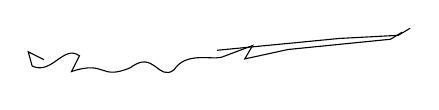
\begin{tikzpicture}[x=1cm,y=1cm]
\draw (0,0.1)--(-0.2,0.2)--(-0.15,0.02)..controls (0.1,-0.1) and (0.25,0.3)..(0.45,0.15)--(0.35,-0.05)..controls (0.8,0.1) and (0.7,-0.17)..(1.1,0)..controls (1.4,0.23) and (1.45,-0.18)..(1.65,-0.03)..controls (1.8,0.2) and (2.1,0.1)..(2.25,0.13)--(2.65,0.28)--(2.55,0.11)--(3.1,0.23)--(3.8,0.3)--(4.4,0.36)--(4.55,0.45);
\draw (2.2,0.22)--(3.75,0.37)--(4.5,0.41)--(4.65,0.5);
\end{tikzpicture}}
Soient $\underline U_0,\underline U'_0$ les ouverts de $\Psi$ induits par $\{0\}\times\Delta^1$, $\Delta^1\times\{0\}$, donc
\[
\left\{\begin{aligned}
\underline U_0&=\{0,a\},\quad\underline U'_0=\{0,b\}\\
\underline U_0\cup\underline U'_0&=\Psi,\quad\underline U_0^{\unsure{\deleted{\prime}}}\cap\underline U'_0=\{0\},
\end{aligned}\right.
\]
on aura donc
\[
\left\{\begin{aligned}
U&=\varphi^{-1}(\underline U_0),\quad U'=\varphi^{-1}(\underline U'_0)\\
U\cap U'&=\varphi^{-1}(\underline U_0\cap\underline U'_0)=\varphi^{-1}(\{0\})=X_0
\end{aligned}\right.
\]
\mspage{42}

\scanpage{44}
90

\textit{sexe est partout dans la psyché} (et que celle-ci le nie et ferme les yeux là où il est n'y change rien), et plus que nulle part ailleurs, il est dans son pouvoir de créer. Et d'autre part, \textit{la psyché et l'âme sont partout dans la réalité.}

Il en est ainsi, tout au moins, et de façon évidente, quand il s'agit de la réalité telle qu'elle est perçue ou conçue par la psyché, c'est-à-dire de la représentation qu'elle se fait de \deleted{\unsure{cette}}\inserted{cette} réalité, de sa relation à elle. Car l'image de la réalité que l'âme se construit aux différents niveaux conscient et inconscients est tout autant et plus une création de l'âme, qu'un simple reflet plus ou moins fidèle d'une ``réalité objective'' qui existerait indépendamment d'elle. (Réalité dont il n'est pas question ici de nier l'existence). C'est dire que \textit{l'état de maturité et les dispositions générales de l'âme déterminent autant et plus son image de la réalité, que cette réalité elle-même ne la détermine.}
\margin{$\cdot$}

Ceci vu, on conçoit qu'un état de peur de l'âme devant elle-même, et de fuite devant la réalité d'elle-même, puisse et doive entraîner une peur et une fuite devant \textit{toute} réalité. Nous pouvons dire aussi que dans notre relation à elle, \textit{toute réalité agit à la façon d'un \textnormal{miroir} dans lequel la psyché voit reflétée une image d'elle-même.} (Et si cette image est rarement perçue au niv\inserted{e}au conscient, elle l'est toujours tout au moins dans l'inconscient profond, y compris dans l'inconscient moyen-profond, où se situe la peur primordiale.) En effet, cette réalité ne peut être distinguée par la psyché de l'image qu'elle s'en fait, c'est-à-dire aussi de sa relation à elle ; et nécessairement et qu'elle le veuille ou non, cette image et cette relation la reflètent.
\margin{$\cdot$}

Cette image de nous-même que nous renvoie la réalité nous implique d'une façon d'autant plus névralgique, et elle déclenche des réactions de peur et de fuite d'autant plus énergiques ou violentes, que cette réalité nous apparaît comme plus ``proche'' de nous. Le plus souvent, ces réactions sont les plus véhémentes ou les plus implacables quand la réalité concerne notre relation soit à nous-même, soit à un être proche : à un parent, \deleted{\unsure{q}}\inserted{a}u conjoint, à \deleted{\unsure{un}}\inserted{notre} enfant - et ceci d'autant plus que la relation est forte, que l'énergie investie en elle est considérable. Mais c'est surtout \textit{la force de notre relation à telle ou telle réalité, l'intensité d'intérêt et l'énergie que nous y investissons, qui sont ici déterminantes.} Ainsi le plus souvent, des spéculations philosophique de haut vol \figure{\begin{tikzpicture}[baseline=-.3ex]\draw[line width=.7pt] (0,0)--(.15,.3);\end{tikzpicture}} aur\deleted{a}\inserted{o}nt beau concerner les questions les plus cruciales (et brûlantes certes !) que l'esprit humain se soit jamais posé sur lui-même, sur Dieu et sur l'âme, ces nobles envolées ne renverront à l'âme qu'une image d'elle pâle voire imperceptible, qui n'aura vertu ni de l'interpeller ni de l'effrayer. Mais même dans une science aussi abstraite et aussi éloignée en apparence de toute réalité humaine que la mathématique, pour peu que notre relation à la belle dame soit ardente et aussitôt elle devient pour nous névralgique, et l'image qu'elle nous renvoie de nous-même forte et véhémente. Et la réaction de peur devant cette image sera d'autant plus viscérale et forte que
\margin{$\cdot$}
\margin{$\cdot$}
\margin{$\cdot\ \cdot$}

\mspage{43}

\scanpage{45}
\mspage{7}

On a aussi
\[U\simeq\unsure{X}_{/a},\quad U'=X_{/b},\quad U\cap U'=X_{/0}.\]
Ainsi le diagramme dans $\mathrm{Cat}$
\[(6)\qquad\diagram{\begin{tikzcd} & U\\ U\cap U'\arrow[ur,"i'_0"]\arrow[dr,"i_0"'] & \\ & U'\end{tikzcd}}\]
du type $\underline\Psi$ n'est-il autre que le foncteur $\underline\Psi\longrightarrow\mathrm{Cat}$ qui définit la cat. \inserted{cofibrée scindée} $\Psi(X/\underline\psi)=\overline X$ sur $\Psi$
\[\diagram{\begin{tikzcd}X\arrow[rr,"\alpha"]\arrow[dr,no head,"\varphi"']&&\overline X\arrow[dl,no head,"\overline\varphi"]\\&\underline\Psi&\end{tikzcd}}\qquad\alpha\in W^{\unsure{g}}_{\underline\Psi}\]
\[U=\overline X_a,\quad U'=\overline X_b,\quad U\cap U'=\overline X_0,\]
les foncteurs $i'_0,i_0$ de (6) étant les foncteurs changement de base relatifs à
\[0\xrightarrow{\underline{i}'_0}a\quad\text{et}\quad0\xrightarrow{\underline{i}_0}b.\qquad\deleted{\text{D'autre}}\]
D'autre part $\overline\varphi$ est \uline{propre}, donc $\overline\varphi_*$ se calcule \unsure{en fibres|fibre} par \unsure{fibres}, en particulier, pour coeff. const. $\xi_{\overline X}$, avec $\xi\in\mathcal A$
\[\overline\varphi_*(\xi_{\overline X})(s)=\begin{cases}H^{\unsure{\bullet}}_{\underline D}(U\cap U',\xi)&\text{si }s=0\\H^{\unsure{\bullet}}_{\underline D}(U,\xi)\deleted{\unsure{*}}&\text{si }s=a\\H^{\unsure{\bullet}}_{\underline D}(U',\xi)&\text{si }s=b.\end{cases}\]
\mspage{44}

\scanpage{46}
\mspage{8}
Donc le diagramme squelettique
\[(*)\quad\diagram{\begin{tikzcd}H^\bullet_{\underline D}(U,\xi)\arrow[dr]&&H_{\underline D}(U',\xi)\arrow[dl,no head]\\&H^\bullet_{\underline D}(U\cap U',\xi)&\end{tikzcd}},\]
\inserted{du type $\underline\Psi^{\mathrm{op}}$,} provient-il d'un diagramme \unsure{concret|ouvert}
\[\sigma_0\deleted{\unsure{\xi_0}}\overset{\mathrm{déf}}=\overline\varphi_*(\unsure{a}_{\overline X})\in\underline D(\underline\Psi).\]
Considérons l'inclusion
\[\underline\Psi\overset{\underline k}{\subset}\deleted{\unsure{*}}\Delta^1\times\Delta^1=\diagram{\begin{tikzcd}&(0,1)\arrow[dr,no head]&\\(0,0)\arrow[ur,no head]\arrow[dr]&&(1,1)\\&(1,0)\arrow[ur]&\end{tikzcd}}\]
déduite de $\Psi$ en lui rajoutant l'élément final manquant $(1,1)$. Soit $\underline k$ l'inclusion, et considérons le ``carré cartésien''
\[\sigma=\underline k_*(\sigma_0)\in\underline D(\Delta^1\times\Delta^1)\]
\deleted{Donc les fibres de $\sigma$ en les points de}
On a
\[\underline k^*(\sigma)\simeq\sigma_0,\]
donc le \deleted{\unsure{fibré diagramme}} squell. induit par $\sigma$ sur $\Psi$ n'est autre que (*), ci-dessus. Mais je dis que le diagramme squelettique sur $\Delta^1\times\Delta^1$ ainsi \inserted{s'identifie :}
\figure{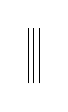
\begin{tikzpicture}\draw (0,0)--(0,.7);\draw (.07,0)--(.07,.7);\draw (.14,0)--(.14,.7);\end{tikzpicture}}
\mspage{45}

\mspage{9}
\[(**)\quad\diagram{\begin{tikzcd}&H^\bullet_{\underline D}(\inserted{\unsure{\overline X|X}},\xi)\arrow[dl,"i^*"']\arrow[dr,"i'^*"]&\\H^\bullet_{\underline D}(U,\xi)\arrow[dr,"i_0'^*"']&&H^\bullet_{\underline D}(U',\xi)\arrow[dl,"i_0^*"]\\&H^\bullet_{\underline D}(U\cap U',\xi)&\end{tikzcd}};\]
\margin{\uline{NB} On a ce carré cartésien, pour $\uline{\forall}\ \xi\in\underline D(\unsure{\overline X|X})$, pas seulement $\xi$ constant\ldots}
Notons pour ceci que si \deleted{\unsure{$\psi$|que}}
\[\psi=\underline k\circ\varphi:\overline X\longrightarrow\Delta^1\times\Delta^1=\underline Q\]
\[\sigma=\underline k_*(\sigma_0)=\underline k_*(\varphi_*(\xi_{\overline X}))=\psi_*(\xi_{\overline X}),\]
d'où
\[H^\bullet_{\underline D}(\Delta^1\times\Delta^1,\sigma)\simeq H^\bullet_{\underline D}(\overline X,\xi)\xrightarrow{\sim}H^\bullet_{\underline D}(X,\xi)\]
\inserted{car $\alpha:X\longrightarrow\overline X$ est $\in W$}
D'autre part, comme $e=(1,1)$ élément final de $\Delta^1\times\Delta^1=\underline Q$ donc $e-\underline Q$ asph.,
\[\deleted{\unsure{\theta}}\qquad\underbrace{H^\bullet_{\underline D}(Q,\sigma)}_{H^\bullet_{\underline D}(\inserted{\unsure{\overline X|X}},\xi)}\simeq\sigma(e)=\sigma(1,1)\deleted{\unsure{\leftarrow\cdots}},\]
d'où l'assertion.
Ça doit faire partie, d'autre part, des propriétés générales des carrés cartésiens \inserted{``dans $\mathcal A$''} (comme (**)), que
\[i_0'^*\text{ iso}\Longleftrightarrow i'^*\text{ iso},\]
\margin{\uuline{à vérifier} (ou à \unsure{mettre en axiome} sur les dérivateurs.)}
\deleted{\unsure{Et}} comme \inserted{ceci} est vrai pour $\uline{\forall}\ \xi\in\mathcal A=\underline De$, cela donne
\[i'_0\in W_{\underline D}\Longrightarrow i'\in W_{\underline D}.\]

\scanpage{47}
\mspage{10}
\deleted{(Donc pour le Dérivateur \deleted{\unsure{fort}}\inserted{``complet''}, avec des coeff. \uline{loc.} constants $\xi$ au lieu de constants, il faut supposer que l'application de pr. $X\longrightarrow\overline X$ est $D$-équiv. $2$-complète.}

Pour avoir l'implication inverse
\[i\in W_{\underline D}\Longrightarrow i_0\in W_{\underline D},\]
il faudrait savoir que le diagramme (**), plus \deleted{\unsure{part}} précisément le \deleted{\unsure{i\longrightarrow}} \deleted{diagramme}\inserted{carré} abstrait $\sigma$ qui lui donne naissance, est non seulement cartésien, mais aussi \uline{cocartésien}. ``Moralement'', qu'il soit cartésien me semble être la traduction cohomologique du fait que le \deleted{diagramme}\inserted{carré}
\[\diagram{\begin{tikzcd}&U\arrow[dl]&\\U\cap U'&&X\arrow[ul,no head]\arrow[dl]\\&U'\arrow[ul]&\end{tikzcd}}\quad\text{dans Cat}\]
est \uline{cocartésien} dans un sens suffisamment fort. Mais il est également cartésien, de façon triviale, et on peut s'attendre (sous certaines conditions) que les diagrammes ``transfigurés'' par $H^\bullet_{\underline D}(-,\xi)$ sont cocartésiens\ldots

J'ai envie de regarder d'emblée $X$ comme sur $\underline Q=\Delta^1\times\Delta^1$, plutôt que sur \unsure{l'ouvert} $\underline\Psi=\underline Q-\{e\}$ de $\underline Q$, alors
\[\underline\Psi_{\underline Q}(X)|\underline\Psi\simeq\Psi_{\underline\Psi}(X)\quad\text{déjà considéré.}\]
\mspage{46}

\scanpage{48}
\mspage{11}
mais la quatrième fibre est
\[\overline X_{(1,1)}=X_{/(1,1)}\simeq X\]
donc le diagramme \inserted{dans Cat} de type $\underline Q$ donnant naissance à $\Psi_{\underline Q}(X)$ n'est autre que
\[\diagram{\begin{tikzcd}&U\arrow[dr,no head]&\\U\cap U'\arrow[ur]\arrow[dr]&&X\\&U'\arrow[ur,no head]&\end{tikzcd}}\]
Mais ce diagramme \inserted{comme ds Cat} n'est bien sûr pas quelconque, sa propriété essentielle, pour les propriétés que nous avons en vue, me semble la suivante :
\[\left(\underbrace{\int\diagram{\begin{tikzcd}&U\\\unsure{V|U\cap U'}\arrow[ur]\arrow[dr,no head]&\\&U'\end{tikzcd}}}_{\substack{\text{déf.}\\\Psi_{\underline\Psi}(X)\text{ en tant}\\\text{qu'objet de Cat sans plus}}}\right)\longrightarrow X\]
\margin{flèche définie pour $\forall$ diagr. comme $\diagram{\begin{tikzcd}&U\arrow[dr,no head]&\\V\arrow[ur]\arrow[dr,no head]&&X\\&U'\arrow[ur]&\end{tikzcd}}$ dans Cat}
est dans $W$. Et le fait général que je \unsure{subodore} est le suivant

``\uline{Principe}'' \unsure{(1)} Soit $\diagram{\begin{tikzcd}&X_a\\X_0\arrow[ur,no head]\arrow[dr,no head]&\\&X_b\end{tikzcd}}$ un diagramme dans Cat du type $\underline\Psi$, soit $\mathcal X$ la cat. cofibrée sur $\underline\Psi$ qu'il définit. Pour tout $\xi$
\margin{\textsf{MédiGraf Montpellier 21999}}
\mspage{47}

\scanpage{49}
\mspage{12}
$\xi\in\underline D(\mathcal X)$,
considérons (si $\varphi:\mathcal X-\underline\Psi$ \unsure{est} la projection)
\[\sigma_0\overset{\mathrm{déf}}=\varphi_*(\xi)\in\underline D(\underline\Psi)\qquad\deleted{\unsure{H}}\]
\[\sigma=\underline k_*(\sigma_0)\in\underline D(\underline Q),\]
donc
\[\begin{aligned}\sigma(0,0)&\simeq\deleted{\unsure{X_0}}H^\bullet_{\underline D}(X_0,\xi)\\\sigma(0,1)&\simeq H^\bullet_{\underline D}(X_a,\xi)\\\sigma(1,0)&\simeq H^\bullet_{\underline D}(X_b,\xi)\\\sigma(1,1)&\simeq H^\bullet_{\underline D}(\mathcal X,\xi)\end{aligned}\]
et \deleted{diagramme} le carré squelettique associé est
\[(*)\quad\diagram{\begin{tikzcd}&H^\bullet_{\underline D}(\mathcal X,\xi)\arrow[dl]\arrow[dr]&\\H^\bullet_{\underline D}(X_a,\xi)\arrow[dr]&&H^\bullet_{\underline D}(X_b,\xi)\arrow[dl]\\&H^\bullet_{\underline D}(X_0,\xi)&\end{tikzcd}}.\]
(NB $\diagram{\begin{tikzcd}&X_a\arrow[dr]&\\X_0\arrow[ur]\arrow[dr]&&\mathcal X\\&X_b\arrow[ur]&\end{tikzcd}}$ n'a rien de carré, dans $\mathcal X$\ldots $X_a\cap X_b=\varnothing$. Mais $\diagram{\begin{tikzcd}&X_{/a}\arrow[dr,no head]&\\X_{/0}\arrow[ur,no head]\arrow[dr,no head]&&\mathcal X\\&X_{/b}\arrow[ur,no head]&\end{tikzcd}}$ est carré, et le carré (*) est aussi déduit de
\mspage{48}

\mspage{13}
celui-là par $H^\bullet_{\underline D}(-,\xi)$.
L'élément $\sigma\in\underline D(\underline Q)$ est cartésien par construction, donc le ``carré'' (*) aussi. Ça serait le cas pour \uline{toute} cat. $\mathcal X$ \inserted{propre} au-dessus de $\underline\Psi$, sans avoir à le supposer cofibré. Mais le fait que $\mathcal X$ soit cofibré doit donner à ce carré la vertu suppl. qu'il est aussi \uline{cocartésien}. J'ai l'impression que ça ne peut absolument pas découler de l'un des axiomes Der 1 -- Der 5,5' vus jusqu'à présent. Je vais le mettre comme

``\uuline{Der 6}'' \inserted{(provisoire)} \deleted{\unsure{Soit}} \inserted{Si} $\mathcal X$ sur $\underline\Psi$ est cofibré, $\xi$ \deleted{\unsure{constant}}\inserted{quelconque} \deleted{\unsure{considéré, les}} de $\underline D(\mathcal X)$, \deleted{\unsure{le}} l'élément
\[\psi_*(\xi)\in\underline D(\underline Q),\]
\margin{où $\psi=(\mathcal X\xrightarrow{\varphi}\underline\Psi\overset{\underline k}{\hookrightarrow}\underline Q)$\\ $\underline Q=\Delta^1\times\Delta^1$}
est non seulement cartésien, mais aussi cocartésien.
\margin{\unsure{à vérifier que ça devient déjà faux} si $\xi$ quelconque (non loc. const.) \unsure{pas} \deleted{\unsure{constant}} \unsure{découle déjà} \unsure{des axiomes antérieurs}.}
\margin{\uline{Axiome des cofibrations}\\\unsure{Sans doute : ceci demande à être explicité en} \unsure{le cas des limites, à l'aide du ``bon'' axiome} \unsure{antérieur} \unsure{Der. 6 de la page qui suit}.}

\scanpage{50}
\mspage{14}
\margin{\deleted{\unsure{formulation fausse}\illegible{1}}}
``\uline{Der 6'}'' \inserted{(provisoire)} Si $\mathcal X$ est fibré sur
\[\underline\Psi^{\mathrm{op}}=\underline\Phi=\left(\diagram{\begin{tikzcd}&a\arrow[dl]\\1&\\&b\arrow[ul]\end{tikzcd}}\right)\]
(donc donné par, à $\underline Q$-équiv. près, par un diagramme $\diagram{\begin{tikzcd}&X_0\\\unsure{X_a|X_1}\arrow[ur,no head]\arrow[dr]&\\&X_b\end{tikzcd}}$ dans Cat) alors pour $\xi\in\underline D(\mathcal X)$ constant (voire l.c.)
\[\deleted{\unsure{H\xi}}\quad\psi_!(\sigma)\in\underline D(\underline Q)\]
est non seulement cocartésien (sans mérites), mais aussi cartésien.
\margin{\uline{Axiome des fibrations}}
\[\underline\Phi\subset\underline Q^{\mathrm{op}}=\diagram{\begin{tikzcd}[row sep=large,column sep=small,execute at end picture={\draw (\tikzcdmatrixname-2-1.center) ++(.45,0) ellipse (.95cm and 1.35cm);}]&a\arrow[dl]&\\1&&0\arrow[ul]\arrow[dl]\\&b\arrow[ul]&\end{tikzcd}}\]
\uline{NB} Der 6' pour $D$ \deleted{\unsure{implique}} n'est autre que Der 6 pour $D^{\mathrm o}$. Je ne vois pas comment l'un impliquerait l'autre, en dehors du cas exceptionnel où il y aurait \deleted{\unsure{comme}\ (\unsure{\forall\xi})} un foncteur dualisant dans $\mathcal A=D(e)$, et une corresp. donnée par dualité entre cohomologie et homologie.

Finalement, il semblerait que le bon axiome, qui englobe Der 6 et Der 6 bis, soit le suivant :
\margin{\uuline{La définition} \deleted{\unsure{abstraite}}}
\margin{``\uuline{l'axiome géométrique}''}
\uline{Der 6} \deleted{\unsure{bis}\illegible{1}} Si $\sigma\in\underline D(\Delta^1\times\Delta^1)$, $\sigma$ est cartésien ssi il est cocartésien.
\inserted{\uline{De plus} (\uline{à moins} que ça \unsure{ne soit absurde}) :}
Le diagramme squelettique associé est
\mspage{49}

\scanpage{51}
\mspage{15}
\[\diagram{\begin{tikzcd}&\sigma(0,1)\arrow[dl,"j_0"']&\\\sigma(0,0)&&\sigma(1,1)\arrow[ul,"i_1"']\arrow[dl,"j_1"]\\&\sigma(1,0)\arrow[ul,"i_0"]&\end{tikzcd}}\]
\unsure{donc} $\begin{cases}i_1\text{ iso}\Longleftrightarrow i_0\text{ iso},\\j_1\text{ iso}\Longleftrightarrow j_0\text{ iso}.\end{cases}$
\margin{De plus, on doit imposer ceci pour les dérivateurs induits $\underline D_I$ ($I\in\unsure{\mathrm{Diag}|\mathrm{Dirg}}$), donc dans $\underline D(I\times\Delta^1\times\Delta^1)$.}

Cette dernière assertion résulte de la précédente (car cart. implique $\Rightarrow$, cocartésien implique $\Leftarrow$), \unsure{prouvons pour ceci} :

``\uline{Lemme}'' \deleted{(associé à Der 6)} : si $\xi=\left(\diagram{\begin{tikzcd}&\xi_a\arrow[dl,"j_0"']\\\xi_0&\\&\xi_b\arrow[ul,"i_0"]\end{tikzcd}}\right)$ est un diagramme abstrait tel que $i_0$ soit un iso, alors il est isom. à l'image inverse d'un $\eta\in\underline D(\underline U)$ \deleted{\unsure{\xi}} (où $\underline U=(\unsure{0}\longrightarrow a)$ \inserted{$\simeq\Delta^1$} est l'ouvert canonique gauche de $\underline\Psi$) par la \unsure{rétraction} $\rho$ de $\underline\Psi$ sur $\underline U$.

Il suffit de prouver que
\[\deleted{\unsure{\xi}}\quad\rho^*\rho_*(\xi)-\xi\qquad\text{l'adj.}\]
est iso. Comme $\rho$ est (\unsure{bien sûr} lisse, comme induit par $\mathrm{pr}_1:\Delta^1\times\Delta^1-\Delta^1$ sur un ouvert) mais aussi \unsure{propre}, $\rho_*(\xi)$ se calcule fibre par fibre. On utilise que \deleted{\unsure{sur}}
\[\mathcal A\simeq\underline D(e)\longrightarrow\underline D^{\mathrm{lc}}(\Delta^1)\]
est une équiv. de cat. (\uline{forme de Der 3})$^*$
\margin{\deleted{\unsure{Il faut raisonner}\illegible{2}\unsure{ici}}}
\mspage{50}

\scanpage{52}
\mspage{16}
Dans Hot, par contre on a ceci :
Tout carré cocartésien est cartésien. Pour qu'un carré cartésien $\diagram{\begin{tikzcd}&\xi_0\arrow[dl,no head]\arrow[dr]&\\\xi_a\arrow[dr,no head]&&\xi_b\arrow[dl,no head]\\&\xi_1&\end{tikzcd}}$ soit aussi cocartésien, il f. et s. que l'on ait
\[\pi_0(\xi_1)=\mathrm{Im}\pi_0(\xi_a)\cup\mathrm{Im}\pi_0(\xi_b)\]
\margin{Complètement faux. Si p.ex. $\xi_1=e$, le diagramme \unsure{n'est-il pas} homotopiquement cartésien et cocartésien que si $\xi_a\simeq e$ \uline{ou} $\xi_b\simeq e$.}
\figure{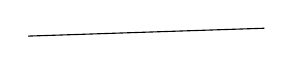
\begin{tikzpicture}\draw (0,0)--(3,.1);\end{tikzpicture}}
Der 6 ou Der 6' entraîne donc W7. Quant à W8, il semble relever d'un principe général

``\uline{Der 8}'' \inserted{(``lemme des cinq'')} Soit un hom. de deux carrés \deleted{\unsure{co}}cartésiens de même nature, dans $\mathcal A(\Delta^1\times\Delta^1)$. Considérons les conditions
\[\diagram{\begin{tikzcd}[row sep=small,column sep=small]
&\xi_a\arrow[dr,no head]\arrow[dddd,"f_a",near start]&\\
\xi_0\arrow[ur]\arrow[dr,no head]\arrow[dddd,"f_0"']\arrow[dddd,no head,shift left=2pt]&&\xi_1\arrow[dddd,"f_1"]\\
&\xi_b\arrow[ur]\arrow[dddd,"f_b",near start]&\\
&&\\
&\eta_a\arrow[dr,no head]&\\
\eta_0\arrow[ur]\arrow[dr]&&\eta_1\\
&\eta_b\arrow[ur]&
\end{tikzcd}}\qquad\begin{array}{ll}a)&f_0\text{ est iso}\\b)&f_1\text{ est iso}\\c)&f_a\text{ et }f_b\text{ sont iso.}\end{array}\]
\deleted{Alors} Si les carrés sont hom. cartésiens, \uline{Alors} \deleted{\unsure{deux de ces trois}} $b+c\Rightarrow a$. S'ils sont hom. cocartésiens, $a+c\Rightarrow b)$. S'ils sont bicartésiens, \deleted{\unsure{cartésiens, ces propriétés}} \deleted{\unsure{le diagramme est}} donc de plus $a+b\Rightarrow c$ (``?'' \unsure{étendre le cas d'un morphisme qui apparaît} \unsure{d'une catégorie}).
\margin{Il suffit d'exiger que $a)+b)\Rightarrow c$, i.e. si $f_0,f_1$ iso, alors $f_a$ et $f_b$ iso, les autres cas \unsure{en découlent}.}
\deleted{\uline{NB} Les deux cas $a+c\Rightarrow b$, $b+c\Rightarrow a$, il suffit cartésien \unsure{dans} et \unsure{l'autre} ci-dessus. Le cas non immédiat est le cas $a+b\Rightarrow c$.}
\mspage{51}

\mspage{17}
\margin{Forme renforcée de W7 p. 9}
\uline{W7 bis} Soit $\diagram{\begin{tikzcd}&X_a\\X_0\arrow[ur,no head]\arrow[dr]&\\&X_b\end{tikzcd}}$ diagramme dans Cat, soit $\underline\Phi=\diagram{\begin{tikzcd}&a\arrow[dl]\\0&\\&b\arrow[ul]\end{tikzcd}}$ et $\mathcal X$ la catégorie fibrée sur $\underline\Phi$ définie par le diagramme. On a un diagramme commutatif dans $\mathrm{Hot}_W$ :
\[\diagram{\begin{tikzcd}&X_0\arrow[dl,"i_a"']\arrow[dr,"i_b"]&\\X_a\arrow[dr,"i'_b"']&&X_b\arrow[dl,"i'_a"]\\&\mathcal X&\end{tikzcd}}\]
\margin{\uline{NB} Autre présentation $\mathcal X$, fibré sur $\diagram{\begin{tikzcd}&a\\0\arrow[ur]\arrow[dr]&\\&b\end{tikzcd}}$. On \uline{part} sur}
(NB Dans Cat, \deleted{je présume que} les deux flèches composées sont homotopes, par un chemin de longueur 2 : elles sont homotopes tous deux, par une homotopie de long. 1, à ``l'inclusion'' $X_0\hookrightarrow\mathcal X$.)
Alors \deleted{\unsure{les}}
\[i_a\in W\Longleftrightarrow i'_a\in W\]
\[i_b\in W\Longleftrightarrow i'_b\in W\]
\margin{(traits pleins)}
\uline{W8 bis} Soit un diagramme comm. dans Cat
\[\diagram{\begin{tikzcd}[row sep=small,column sep=small]
&X_a\arrow[dr,dashed]\arrow[dddd,"f_a",near start]&\\
X_0\arrow[ur,no head]\arrow[dr,no head]\arrow[dddd,"f_0"']&&\mathcal X\arrow[dddd,"f"]\\
&X_b\arrow[ur,dashed]\arrow[dddd,"f_b",near start]&\\
&&\\
&X'_a\arrow[dr,dashed]&\\
X'_0\arrow[ur,no head]\arrow[dr,no head]&&\mathcal X'\\
&X'_b\arrow[ur,dashed]&
\end{tikzcd}}\]
\margin{Équivalent : l'énoncé dans $\mathcal X,\mathcal X'$ cofibrées sur $\underline\Psi$, avec hom \uuline{cartésien} $\mathcal X\longrightarrow\mathcal X'$.}
\margin{Cet axiome, \unsure{c'est donc} W7 bis, à l'hyp. $f$ cartésien (\unsure{W8 bis}) \unsure{est déjà}\illegible{2}\unsure{équivalent}.}
se complète par un diagramme commutatif dans $\mathrm{Hot}_W$ (déf. construction de $\mathcal X,\mathcal X'$ comme $\mathcal X=\int(\diagram{\begin{tikzcd}&X_a\\X_0\arrow[ur,no head]\arrow[dr]&\\&X_b\end{tikzcd}})$). Considérons les cond.
\[\begin{cases}a)\quad\unsure{f|f_a}\in W\\b)\quad f_0\in W\\c)\quad f_a\text{ et }f_b\in W\end{cases}\]
Alors deux de ces conditions entraînent la troisième.

\scanpage{53}
\mspage{18}
\deleted{Version forte}\inserted{Corollaire de W7 bis} (\deleted{\unsure{W8}} forme plus forte en apparence)
\uline{W7 \unsure{ter|bis}} Soit $\mathcal X$ lisse sur $\Phi=\diagram{\begin{tikzcd}&a\arrow[dl]\\0\arrow[dr]&\\&b\end{tikzcd}}$, d'où diagramme (comm. dans $\mathrm{Hot}_W$)
\[\diagram{\begin{tikzcd}&X&\\X_a\arrow[ur,"i'_b"]&&X_b\arrow[ul,"i'_a"']\\&X_0\arrow[ul,"i_a"]\arrow[ur,"i_b"']&\end{tikzcd}}\]
Alors
\[i_a\in W\Longleftrightarrow\unsure{i'_a|i'_0}\in W\]
\[(\text{donc }i_b\in W\Longleftrightarrow i'_b\in W)\]
(NB Cela implique l'énoncé dual W7' ter, avec $X$ propre sur $\Psi=\diagram{\begin{tikzcd}&a\arrow[dl]\\0&\\&b\arrow[ul]\end{tikzcd}}$)

Corollaire de W8 bis (forme renforcée en apparence).
\uline{W8 \unsure{ter|bis}} Soient $\mathcal X,\mathcal X'$ lisses sur $\underline\Phi=\diagram{\begin{tikzcd}&a\arrow[dl]\\0&\\&b\arrow[ul]\end{tikzcd}}$, et $f:\mathcal X-\mathcal X'$ un $\underline\Phi$-morphisme. Soient $f_a,f_b,f_0$ induits sur les fibres, et les conditions
\[\begin{array}{ll}a)&f\in W\\b)&f_0\in W\\c)&f_a\text{ et }f_b\in W\end{array}\]
Alors deux de ces conditions impliquent la troisième.
\mspage{52}

